%% Chapter 13 — MLOps와 배포 자동화
\setcounter{chapter}{12}
\chapter{MLOps와 배포 자동화}
\chaptersubtitle{레지스트리, 파이프라인, 카나리, 섀도 — 배포가 엔지니어링에서 가장 지루한 문장이 되는 법}

\begin{calloutbox}{tbbblue}{tbbbluefill}
{\normalsize\bfseries\color{tbbblue}학습 목표}\par\vspace{3pt}
\begin{tbbitemize}
  \item 잘못된 배포를 개인의 부주의가 아니라 \textbf{빠진 제도}(버전이 있는 릴리스, 파이프라인, 점진적 노출)의 문제로 진단하고 피해 사용자-분 수치로 차이의 가격을 계산한다.
  \item \textbf{모델 레지스트리}를 운영한다. 릴리스 삼중항(가중치 + 설정 + 이미지 다이제스트), 게이트 증거, 계보, 단계 별칭을 관리하고 롤백을 연습된 포인터 전환으로 수행한다.
  \item \textbf{모델 CI/CD}를 구축한다. 세 경로(PR 검사, 병합 후 레지스트리 등록, 카나리와 함께 승격), 모델 CI와 앱 CI의 차이, 자체 호스팅 GPU 러너를 포함한 GitHub Actions 메커니즘을 이해한다.
  \item 각각이 \textbf{답하는 질문}에 따라 배포 전략을 선택한다. 롤링은 "부팅되는가?", 블루/그린은 "즉시 되돌릴 수 있는가?", 카나리는 "고장 났는가?", A/B는 "더 나은가?", 섀도는 "무엇을 했을 것인가?"에 답한다.
  \item 생성 모델의 \textbf{카나리 분석}을 설계한다. SLO 조항과 가드레일 프록시, 세션 일관적 분할, 자동 승격/자동 후퇴를 포함하고 오프라인 게이트가 확인할 수 없는 무엇을 검사하는지 설명한다.
  \item \textbf{관리형 엔드포인트}(SageMaker, Vertex AI)를 오퍼레이터 사다리 위에 배치하고, 무엇을 실행하고 어떤 비용을 청구하며 무엇은 언제나 사용자 몫인지 파악한다.
\end{tbbitemize}
\end{calloutbox}

\vspace{2.5pt}

\begin{calloutbox}{tbbteal}{tbbtealfill}
{\normalsize\bfseries\color{tbbteal}핵심 용어}\par\vspace{3pt}
피해 사용자-분 · 모델 레지스트리 · 릴리스 삼중항 · 계보 · 단계 별칭 · 승격 / 롤백 · CI/CD · GitHub Actions · 자체 호스팅 러너 · OIDC · 골든 요청 · 빠른 게이트 대 전체 게이트 · 점진적 전달 · 롤링 · 블루/그린 · 카나리 · 자동 분석 · 가드레일 메트릭 · A/B 테스트 · 섀도 / 다크 론치 · Argo Rollouts · 관리형 엔드포인트 · 배포 가드레일 · DORA 메트릭
\end{calloutbox}

\vspace{2.5pt}

\begin{calloutbox}{tbblightgray}{tbbboxfill}
{\normalsize\bfseries\color{tbbink}장 구성}\par\vspace{3pt}
\textbf{13.1} 금요일 배포 — 역사상 가장 비싼 누락 서버    \textbf{13.2} 레지스트리: 의미 있는 버전    \textbf{13.3} 파이프라인: 모든 약속을 장치가 검사한다    \textbf{13.4} 실제 트래픽과 만나기: 롤링, 블루/그린, 카나리, A/B, 섀도    \textbf{13.5} 관리형 엔드포인트: 완성된 오퍼레이터 사다리    \textbf{13.6} 실습: 파이프라인을 만들고 프로덕션을 깨뜨리는 데 실패하기 — 이어서 요약, 연습문제, 더 읽을거리
\end{calloutbox}

\section{금요일 배포 — 역사상 가장 비싼 누락 서버}

제12장은 정직하게 부끄러운 장면으로 끝났다. 플릿은 숨 쉬고 청구서는 마감되었지만, 모든 개선을 \textbf{사람이 노트북에서 kubectl을 입력해} 배포했다. 이 교재는 몇 주 동안 다이제스트, 저장소, 게이트, 프로브, 카나리 필드라는 대안을 조용히 쌓아 왔다. 하지만 아직 조각을 조립하지 않았고 조립되지 않은 조각은 누구도 보호하지 못한다. 현재 팀이 세부까지 그대로 재현할 수 있는 금요일 저녁 6시의 모습은 다음과 같다.

\begin{terminalbox}
\begin{Verbatim}[breaklines=true,breakanywhere=true,fontsize=\small,formatcom=\color{tbbtermfg},codes=\tbbcodeactive]
# friday 18:07. v10-awq passed the offline gate this afternoon.
$ kubectl set env deploy/chat MODEL_URI=s3://models/chat/v10-awq/
# 18:12  rolling update complete. probes green. weekend, here we come.
# 18:19  support: "answers keep cutting off mid-sentence??"
$ kubectl get pods; curl :8000/metrics | grep -E "ttft|error"
#        pods Ready. TTFT p99 0.44s. errors 0.0%. ...all GREEN.
# 18:31  more tickets. decision: roll back. ...roll back to WHAT?
$ history | grep MODEL_URI      # archaeology. Slack. more grep.
# 18:43  found it: v9-int4. re-deploy. 18:56: healthy.
#
# the bug: v10's bundled generation_config.json shipped
# max_tokens: 256 (v9: 1024). the model was FINE. the gate never
# noticed - it scores teacher-forced eval, it never GENERATES.
# damage: 37 minutes x 100% of users. mean answer: 211 -> 54 tokens.
\end{Verbatim}
\end{terminalbox}
\figcaption{사례 13-A  금요일 배포. 충돌한 것은 없고 모든 대시보드는 녹색이며 모델 자체도 완벽했다. 릴리스 밖에서 이동한 설정 파일 하나가 37분 동안 모든 답변 길이를 4분의 1로 잘랐다. 아무도 "이전"이 무엇인지 말할 수 없어 롤백에는 셸 기록을 발굴하는 12분이 걸렸다.}

조직이 가장 먼저 제시할 \textit{"엔지니어가 max\_tokens를 확인했어야 한다"}는 진단을 경계하라. 사실이지만 쓸모가 없다. 개인은 대략 일정한 비율로 실수하고 각 실수의 비용은 시스템이 결정한다. 판사가 아니라 감사인의 눈으로 사례를 다시 읽으면 세 가지 \textbf{빠진 제도}가 보인다. \textit{"이전에 무엇이 실행 중이었는가?"}에 12분 안에 답하지 못한 것은 \textbf{버전 관리} 실패다. 저장소에는 불변 바이트가 있었지만 어떤 바이트와 설정이 실행 릴리스를 구성했는지 기록하지 않았다. 게이트는 모델 점수를 계산했지만 \textit{배포 설정으로 생성해 보지 않았다.} 이는 \textbf{파이프라인} 실패다. 배포된 산출물이 아니라 확인하기 편한 대상을 검사했다. v10이 첫 1초부터 사용자 100\%를 만난 것은 \textbf{노출} 실패다. 현실과 점진적으로 접촉하지 않았고 자동 후퇴도 없었다. 엔지니어만 고치면 다른 엔지니어와 같은 금요일이 반복된다. 세 제도를 고치면 금요일은 그림 13-1의 두 번째 시간선이 된다. 같은 버그를 10\% 카나리의 답변 길이 가드레일이 5분 안에 잡고 자동 후퇴하며 PR에 증거를 기록한다. \textbf{피해 사용자-분이 37에서 0.5로} 74× 줄고 누구의 주말도 희생하지 않는다.

\begin{tbbfigure}
  \adjustbox{max width=0.94\linewidth,max totalheight=0.46\textheight}{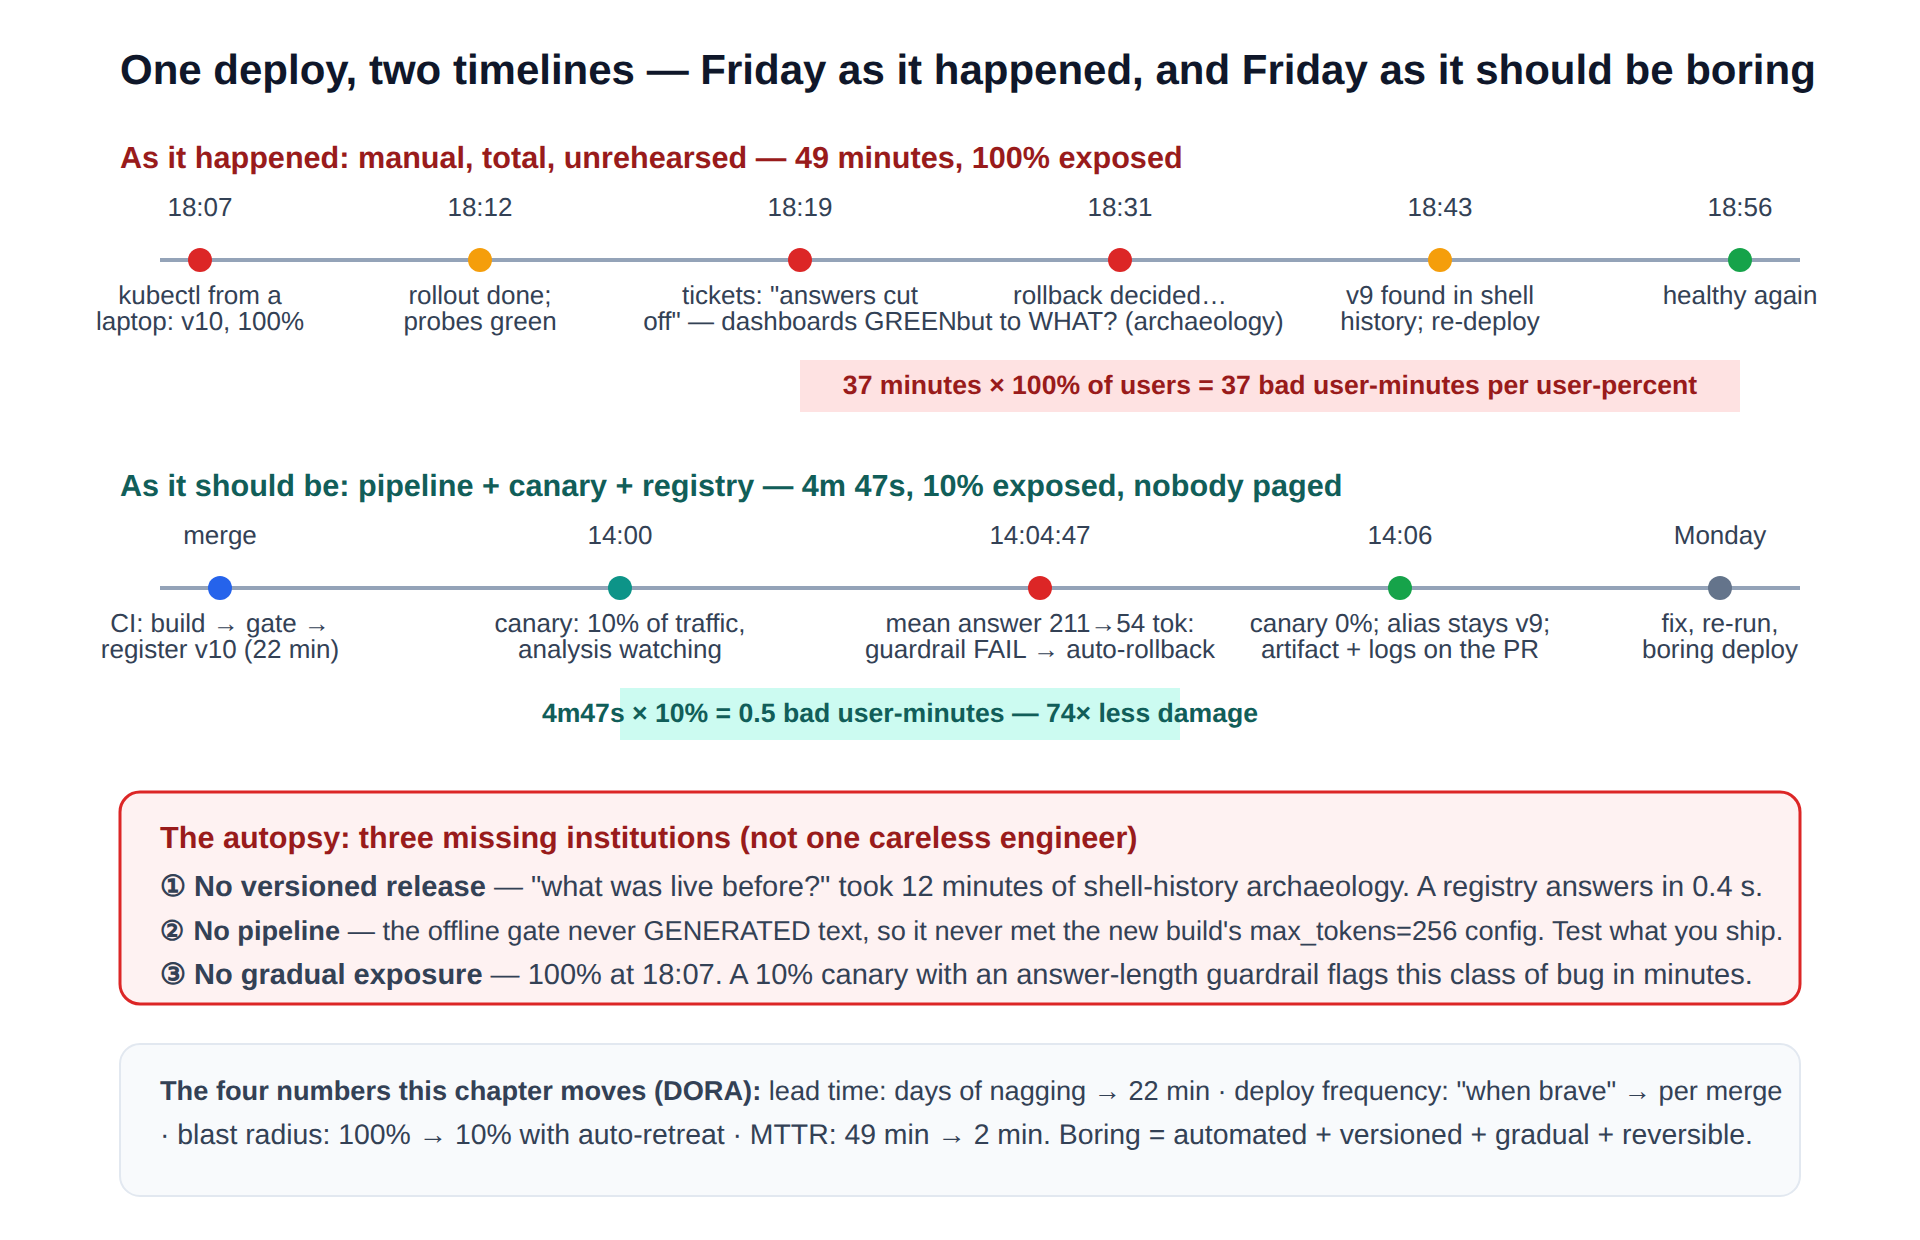
\includegraphics{figures/fig13-1_friday.png}}\\[3pt]
  \figcaption{그림 13-1  배포 하나와 두 시간선. 수동/전체/연습 없음은 사용자 전체에 49분간 영향을 준다. 파이프라인/카나리/레지스트리는 사용자 열 명 중 한 명에게 4m47s 동안 노출한 뒤 자동 후퇴하고 증거를 첨부한다. 이 장은 두 행 사이의 거리를 다룬다.}
\end{tbbfigure}

\subsection*{2012년 8월 1일: 45분과 4억 6천만 달러}

사례 13-A가 견딜 만해 보인다면 실제로 그랬다. 산업 역사는 견딜 수 없었던 버전을 제공하며, 이 장의 규율을 대표하는 사례이므로 두 문단을 할애할 가치가 있다. \textbf{Knight Capital}은 미국 주식 시장 최대 마켓 메이커 중 하나였고 평소 미국 주식 약 열 주 중 한 주를 거래했다. NYSE 출시 기한을 맞추려고 엔지니어가 새 주문 라우팅 코드를 회사의 \textbf{프로덕션 서버 여덟 대에 수동으로 배포하다가 한 대를 빠뜨렸다.} 새 릴리스는 오래된 기능 플래그를 재사용했다. 업데이트하지 않은 여덟째 서버에서 이 플래그는 여전히 \textbf{2003년의 죽은 코드}를 가리켰다. 다른 시스템을 실습 환경에서 시험하려고 의도적으로 비싸게 사고 싸게 파는 Power Peg라는 테스트 모듈이었다. 2012년 8월 1일 시장이 열리자 플래그가 활성화되었다. 서버 일곱 대는 새 코드를 실행했고 여덟째 서버는 좀비를 깨웠다. \textbf{45분} 동안 154개 종목에 의도하지 않은 주문 수백만 건을 냈다. 손실은 약 \textbf{\$460 million}, 초당 약 \$170,000였고 회사 시가총액은 \textasciitilde{}\$1 billion이었다. 이후 SEC 명령은 이 장의 절 제목이 빠져 있는 목록과 같다. 자동화되고 검증된 배포가 없었다. \textit{사람}이 서버 여덟 대에 푸시했고 \textit{장치}는 8/8을 확인하지 않았다. 배포의 두 번째 검토도 없었다. 재사용 플래그가 새 동작을 버전 없는 죽은 코드에 연결했고 킬 스위치(kill switch)도 없었다. 반드시 기억할 세부는 \textbf{시스템이 피를 흘리는 동안 어디에서 무엇이 실행되는지 아무도 확신하지 못했다}는 것이다. 그래서 첫 "수정"은 플래그를 켜 둔 채 정상 서버 일곱 대의 \textit{새} 코드를 롤백해 상황을 \textit{악화}시켰다. Knight는 1년 안에 사실상 사라져 경쟁사에 흡수되었다.

업계의 긍정적인 극은 재난보다 먼저 등장해 대비가 더 선명하다. 2009년 Flickr의 두 엔지니어 John Allspaw와 Paul Hammond는 청중 대부분에게 오타처럼 들리는 제목으로 발표했다. \textbf{"10+ Deploys per Day."} 전체 DevOps 운동의 씨앗이 된 주장은 배포가 위험하므로 \textit{드물어야 한다}는 당시 직관을 뒤집었다. 배포가 위험하므로 \textbf{작고 자동화되며 관찰 가능하고 지속적이어야 한다.} 드문 배포는 큰 배포이고, 큰 배포는 연습하지 않은 중대한 사건이며, 연습하지 않은 중대한 사건이 Knight Capital이다. 이후 15년간의 업계 측정인 \textbf{DORA} 연구 프로그램이 이 역전을 정량화했다. \textit{가장 자주} 배포하는 팀이 변경 실패율도 \textit{가장 낮고} 복구도 가장 빠르다. 빈도가 이 장에서 구축할 메커니즘을 강제하기 때문이다. 목표 상태는 네 수치로 요약되며 그림 13-1 아래 띠가 교재 프로젝트에 맞게 가격을 매긴다. 병합부터 프로덕션까지 \textbf{리드 타임}은 며칠간 독촉하던 상태에서 22분 파이프라인으로, \textbf{배포 빈도}는 "누군가 용감할 때"에서 모든 병합으로, \textbf{변경 실패 장애 반경}은 사용자 100\%에서 자동 후퇴하는 10\% 카나리로, \textbf{복구 시간}은 49분간 발굴하던 상태에서 2분 별칭 전환으로 바뀐다. 이 장의 논지는 한 문장이다. \textbf{배포는 자동화되고 버전이 있으며 점진적이고 되돌릴 수 있는 만큼 정확히 지루해진다.} 지루함은 운영이 줄 수 있는 최고의 칭찬이다.

앞으로 90분의 지도를 보자. 각 절이 하나의 제도를 만든다. \textbf{§13.2}는 \textit{기억}을 만든다. 제6장의 저장소 위에 레지스트리를 두고, 릴리스를 게이트 보고서가 붙은 다이제스트 삼중항으로 정의하며, 승격은 별칭 전환이 된다. "이전에 무엇이 실행 중이었는가?"는 0.4초 쿼리로 답한다. \textbf{§13.3}은 \textit{반사 작용}을 만든다. 세 경로의 GitHub Actions 파이프라인이 모든 후보에서 교재의 모든 게이트인 제7장의 동등성, 제10장의 허용 오차, 제9장의 스윕을 동일하게 실행하고 큰 소리로 거부한다. \textbf{§13.4}는 \textit{신중함}을 만든다. 롤링부터 카나리, 섀도까지 점진적 전달을 다루고 카나리 자동 분석으로 제12장이 남긴 질문에 답한다. 실제 트래픽은 게이트가 확인할 수 없는 무엇을 검사하는가? \textbf{§13.5}에서는 이 메커니즘 대부분을 서비스로 판매하는 \textbf{관리형 엔드포인트}(SageMaker, Vertex)를 살펴본다. 개념은 같고 YAML은 다르며 마진이 붙는다. \textbf{§13.6}은 파이프라인을 만든 뒤 게이트와 카나리에서 한 번씩, \textit{프로덕션을 두 번 깨뜨리는 데 실패}해 점수를 얻는 실습이다. 배포는 지루하지만 거기까지 가는 과정은 그렇지 않다.

\begin{calloutbox}{tbbpurple}{tbbpurplefill}
{\normalsize\bfseries\color{tbbpurple}생각해 보기}\par\vspace{3pt}
\begin{tbbitemize}
  \item 사례 13-A의 대시보드는 사고 내내 녹색이었다. TTFT, TPOT, 오류가 모두 정상이었다. 제7/11장을 이용해 교재의 전체 메트릭 용어가 이 버그를 놓치는 이유와 이를 잡을 수 있는 가장 작은 새 메트릭을 설명하라. 방금 가드레일 메트릭을 발명했으니 §13.4까지 기억해 두자.
  \item Knight의 첫 대응자는 \textit{새} 코드를 롤백해 상황을 악화시켰다. 실제 트리거는 여덟째 서버의 재사용 \textit{플래그}였기 때문이다. 이 장의 용어로 실패를 다시 설명하라. "릴리스"는 무엇이었고 무엇에 버전이 있었으며 무엇에는 없었는가? "어디에서 무엇이 실행되는가"를 추측이 아니라 쿼리로 만들었을 §13.2의 산출물도 제시하라.
  \item 반대 문화를 가장 강한 형태로 논증하라. 한 은행은 2주 검토 게이트를 거쳐 위험 모델을 분기마다 배포한다. DORA의 논리로 드물고 무거운 방식이 올바른 체제인 경우가 있는지 논하고, 은행과 Flickr를 화해시키는 숨은 변수인 배포당 변경 배치 크기를 찾아라.
  \item 사례 13-A의 세 세계에서 피해 사용자-분을 계산하라. (a) 실제 상황, (b) 10\% 카나리로 5분 안에 감지, (c) 출시 전에 잡는 섀도 모드(노출 0\%)다. 각 세계는 추가 메커니즘에 어떤 비용을 냈으며 교재 프로젝트에는 무엇을 가장 먼저 구축할 것인가?
\end{tbbitemize}
\end{calloutbox}

\section{레지스트리: 의미 있는 버전}

제6장은 멋진 선반을 만들고 13주 차에 사서를 세우겠다고 했다. 저장소는 \textit{바이트} 문제를 해결했다. 깔끔한 접두사 아래에 불변 버전을 두고, 다이제스트로 신원을 식별하며, 병렬로 로드하고, 데이터셋과 골든 픽스처도 나란히 놓았다. 하지만 객체 더미라는 구조로는 새벽 2시에 중요한 유일한 질문에 답할 수 없다. \textbf{어느 버전이 실행 중인가? 어느 버전으로 안전하게 롤백할 수 있는가? 누가 무엇을 기준으로 검사했고 누가 승인했는가?} 금요일에 12분간 발굴한 것은 파일 시스템에 거버넌스 질문을 던진 대가였다. \textbf{모델 레지스트리}는 답을 주는 데이터베이스다. 작고 지루하지만 시스템을 지탱하는 \textit{바이트에 대한 약속}의 카탈로그다. 특정 공급업체 화면이 아니라 개념으로 스키마를 배워야 한다. MLflow, Weights \& Biases, SageMaker와 Vertex의 내장 기능 등 여러 로고를 달고 만나게 되며, JSON만으로 오후 한 번에 쓸 만한 것을 직접 만들 수도 있다.

\begin{tbbfigure}
  \adjustbox{max width=0.94\linewidth,max totalheight=0.46\textheight}{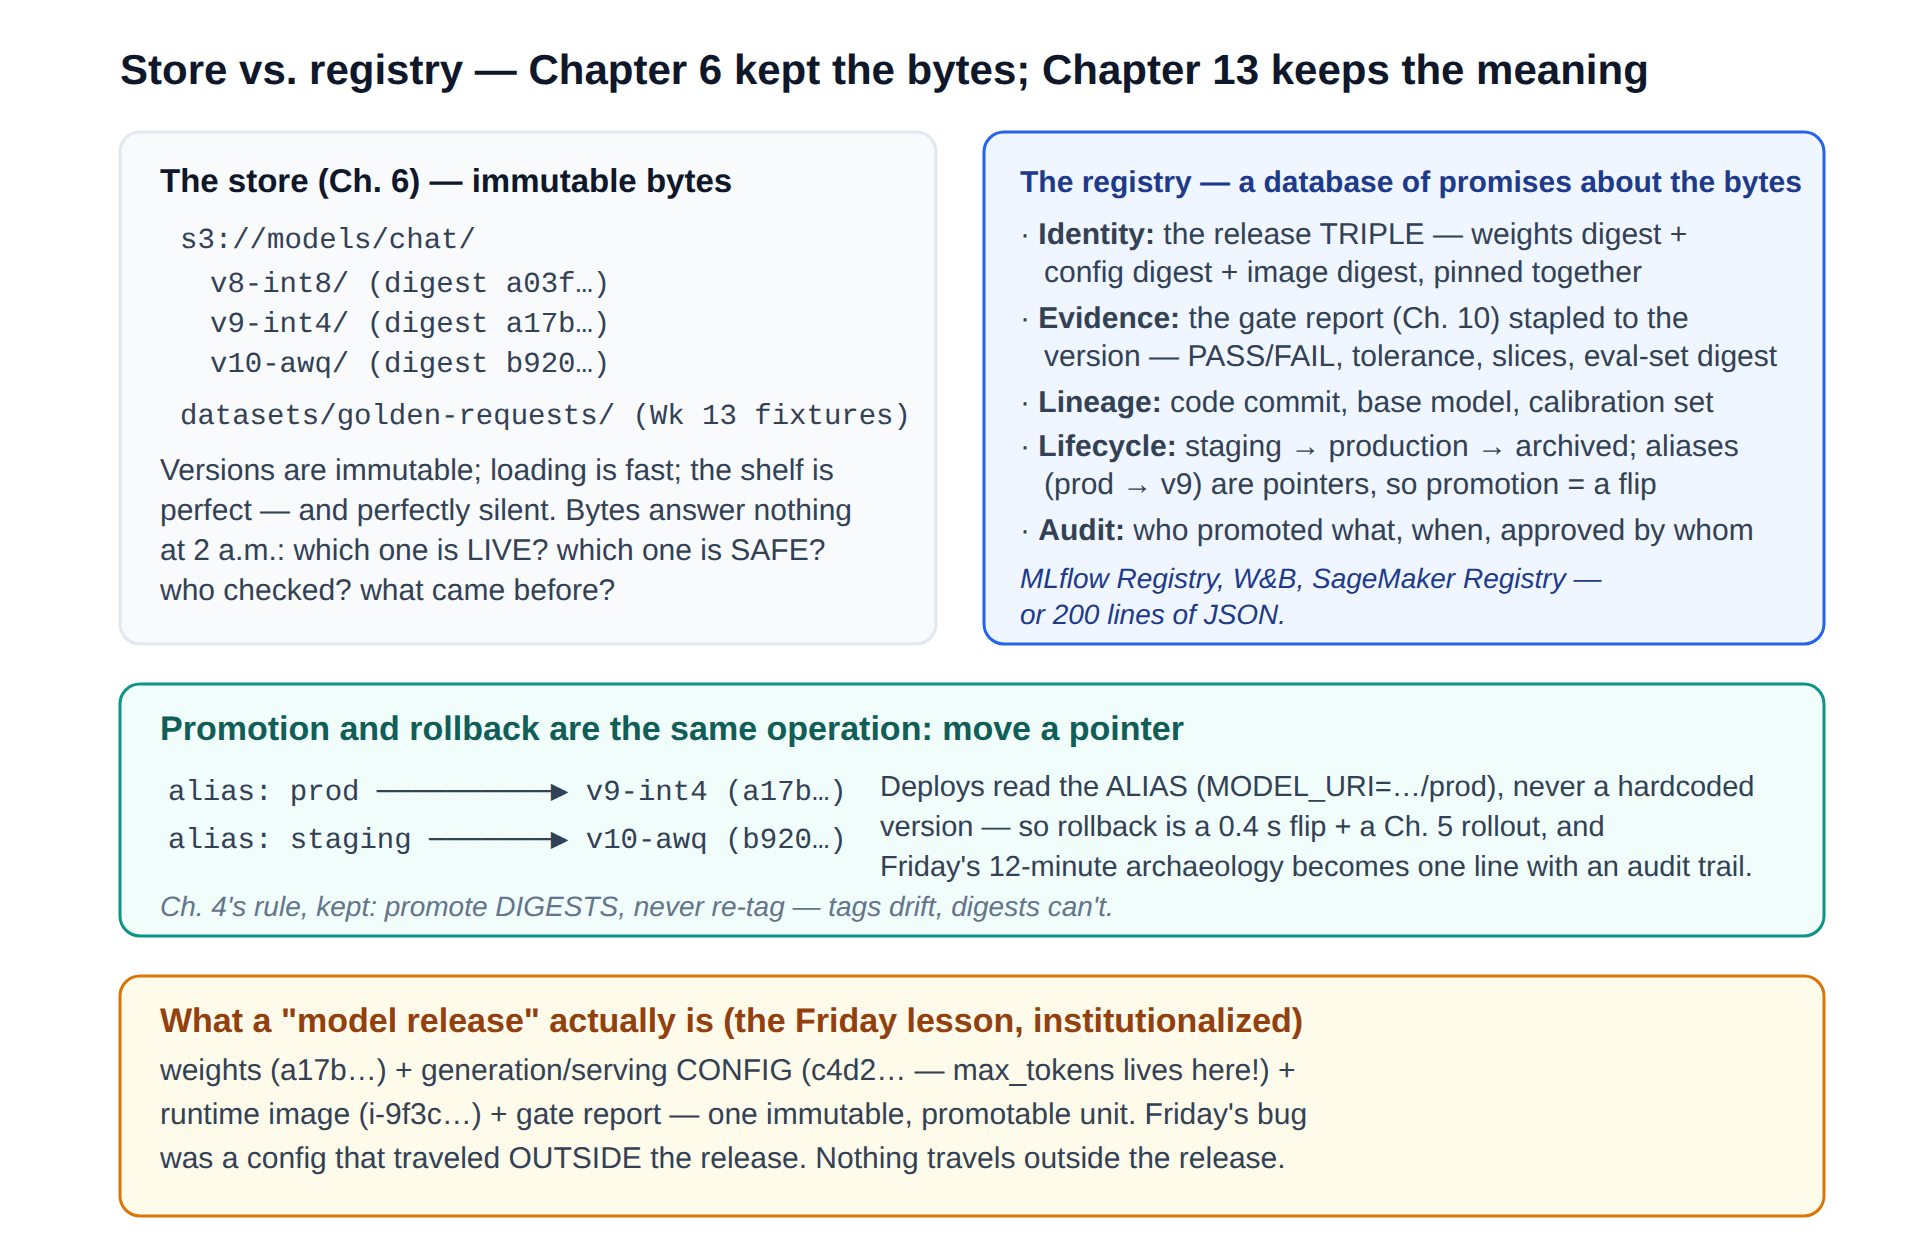
\includegraphics{figures/fig13-2_registry.png}}\\[3pt]
  \figcaption{그림 13-2  저장소 대 레지스트리. 저장소는 불변 바이트를 보관하고 레지스트리는 신원(릴리스 삼중항), 증거(게이트 보고서), 계보, 수명 주기(별칭), 감사를 보관한다. 승격과 롤백은 포인터를 옮기는 같은 작업이다.}
\end{tbbfigure}

\subsection*{릴리스 삼중항 — 금요일 버그를 구조적으로 불가능하게 만들기}

레지스트리의 원자는 "모델 하나"가 아니라 \textbf{릴리스}다. \textit{함께 요청에 답하는 완전하고 불변인 산출물 집합}을 뜻한다. 교재 서비스에서는 \textbf{다이제스트 삼중항}이다. 가중치(제6장의 접두사, 다이제스트 \code{a17b…}), max\_tokens, 템플릿, 표본 추출 기본값이 있는 서빙/생성 \textbf{설정}(\code{c4d2…}), 런타임 \textbf{이미지}(\code{i-9f3c…}, 제4장)다. 하나의 버전 번호 아래 셋을 함께 고정하면 금요일의 실패 유형이 구조적으로 사라진다. \textit{릴리스란 함께 이동하는 것이라고 정의}했으므로 설정이 "릴리스 밖에서 이동"할 수 없다. 물려받은 두 규율이 원자를 신뢰할 수 있게 한다. 제4장의 \textbf{다이제스트를 승격하고 다시 태그하지 않는다}는 규칙이 첫째다. 그 장의 생각해 볼 문제는 이유를 물었고 이제 답을 체감할 수 있다. 다시 푸시한 \code{prod} 같은 태그는 발밑에서 의미가 바뀌는 이름이다. Knight의 여덟째 서버는 돈이 걸린 태그 드리프트의 모습이다. 다이제스트는 드리프트할 수 없다. 둘째는 제10장의 \textbf{게이트 보고서를 버전에 붙인다}는 규칙이다. PASS/FAIL, 허용 오차, 슬라이스 표, 평가 세트 자체의 다이제스트를 포함한다. 그러면 "v10은 안전한가?"는 회의가 아니라 조회가 된다.

\subsection*{별칭: 포인터로 승격하고 연습한 대로 롤백하기}

두 번째 아이디어는 컴퓨팅보다 오래된 \textbf{간접 참조}다. 배포는 버전을 직접 참조하지 않는다. 제6장의 \code{MODEL\_URI}는 \textbf{별칭}(\code{…/\allowbreak chat/\allowbreak prod})을 가리키고 레지스트리가 별칭을 버전에 대응시킨다. 승격은 포인터 이동(\code{prod: v9 → v10})이고 롤백은 같은 이동의 반대 방향이다. 둘 다 원자적이고 로그에 기록되며 1초보다 훨씬 짧게 걸린다. 이후 플릿은 5주 차부터 신뢰해 온 제5장의 일반 롤아웃, 즉 추가 파드, 프로브, 준비 상태 게이팅으로 수렴하거나 다음 파드 탄생 시 별칭을 다시 해석한다. 새벽 2시 이야기가 어떻게 달라지는지 보자. \textit{결정}("v9으로 돌아간다"), \textit{지식}("v9은 게이트를 통과하고 프로덕션에서 11일간 서빙한 마지막 버전이다"), \textit{메커니즘}(명령 하나)이 이제 연습된 상태로 한곳에 있다. 실습에서 시간을 재면 \textbf{별칭 전환 0.4 s, 플릿 수렴 \textasciitilde{}2 minutes}다. §12.3의 탄생 계산에 따라 롤백 하한은 콜드 스타트이며 이를 줄이는 연습을 한 이유다. 수명 주기 단계(staging → production → archived)는 규칙이 붙은 구별된 별칭일 뿐이다. 게이트 보고서, 승인 기록, §13.4 이후에는 카나리 판정이 없으면 아무것도 \code{production}에 도달하지 못한다.

\begin{terminalbox}
\begin{Verbatim}[breaklines=true,breakanywhere=true,fontsize=\small,formatcom=\color{tbbtermfg},codes=\tbbcodeactive]
$ python registry.py list chat
 ver  stage       weights        config   image     gate        by
 v8   archived    a03f…/int8     c11e…    i-77aa…   PASS 09-28  jslee
 v9   production  a17b…/int4     c4d2…    i-9f3c…   PASS 10-05  minj
 v10  staging     b920…/awq      c9aa…    i-2be1…   PASS 10-12  CI

$ python registry.py show chat/v10 --lineage
 commit 8d31f2  base Qwen2.5-3B  calib calib-2026-10a (digest 77e1…)
 eval-set golden-v4 (digest 3c9d…)  gate: delta -0.18pt (tol 0.5) PASS

$ python registry.py rollback chat --to v9        # the 2 a.m. one-liner
alias prod: v10 -> v9   (flip 0.4s; fleet converges via rollout)
audit: 2026-10-12T02:13Z rollback by oncall-kim, reason="ans-len"
\end{Verbatim}
\end{terminalbox}
\figcaption{기록 13-1  직접 사용한 레지스트리. 금요일에 답하지 못한 세 질문인 무엇이 실행 중이고 무엇이 안전하며 무엇이 바뀌었는지를 각각 한 줄로 답한다. 롤백은 승격과 같은 메커니즘이므로 지루해질 때까지 연습할 수 있다.}

\subsection*{무엇이 버전을 올리는가 — 변경 분류 체계}

팀은 겉보기에는 작은 질문에서 멈추곤 한다. \textit{어떤 변경에 새 버전이 필요한가?} 레지스트리의 답은 기계적이다. \textbf{삼중항에서 어떤 다이제스트든 바뀌면 무조건 새 릴리스다.} 하지만 변경 클래스마다 \textit{결과}가 다르므로 한 번 적어 두면 반복되는 논쟁을 끝낼 수 있다. 두 가지 미묘한 경우를 따로 짚자. \textbf{설정 전용 릴리스}는 금요일의 수정처럼 같은 가중치에 \code{max\_tokens}만 고친 경우다. 실제 릴리스이므로 새 버전과 새 게이트 실행이 필요하지만 게이트의 \textit{범위}를 줄일 수 있다. 가중치가 같으면 동등성 검사는 의미가 없지만, 금요일 문제가 설정에 있었으므로 골든 요청과 가드레일 기준선 등 생성에 관련된 모든 검사를 다시 실행해야 한다. \textbf{평가 세트 변경}은 더 교묘하다. 릴리스를 전혀 만들지 않으면서 이후 모든 판정의 의미를 조용히 다시 정의한다. 그래서 평가 세트도 코드처럼 버전 관리(golden-v4 → golden-v5, 다이제스트 고정)한다. 기존 게이트 보고서는 사용한 세트의 이름을 계속 남기고, 세트 변경 후 첫 실행은 비교하지 않고 \textit{기준선을 다시 설정}한다. 어느 시험인지 모르면 성적에는 의미가 없다.

\begin{tbbtablewrap}
  \begin{tabular}{@{}>{\raggedright\arraybackslash}m{\dimexpr 0.2500\tbltextwidth-2\tabcolsep\relax} >{\raggedright\arraybackslash}m{\dimexpr 0.2287\tbltextwidth-2\tabcolsep\relax} >{\raggedright\arraybackslash}m{\dimexpr 0.2660\tbltextwidth-2\tabcolsep\relax} >{\raggedright\arraybackslash}m{\dimexpr 0.2553\tbltextwidth-2\tabcolsep\relax}@{}}
  \arrayrulecolor{tbbnavy}\specialrule{1pt}{0pt}{0pt}
  \rowcolor{tbbtablehead}{\centering \bfseries\color{tbbnavy}변경} & {\centering \bfseries\color{tbbnavy}새 릴리스?} & {\centering \bfseries\color{tbbnavy}다시 실행할 항목} & {\centering \bfseries\color{tbbnavy}일반적인 전략(§13.4)} \\
  \arrayrulecolor{tbbnavy}\specialrule{0.7pt}{0pt}{2pt}
  {\textbf{새 가중치(재학습/양자화)}} & {예 — 새 삼중항} & {전체: 동등성, 게이트, 스윕, 카나리} & {카나리. 모델 계열 경계에서는 섀도} \\
  \arrayrulecolor{tbbtableborder}\hline
  {\textbf{설정만(표본 추출, 토큰)}} & {예 — 설정 다이제스트} & {생성 경로 검사: 골든 요청, 가드레일 기준선, 카나리} & {카나리(금요일 유형이 여기 있다!)} \\
  \arrayrulecolor{tbbtableborder}\hline
  {\textbf{이미지만(의존성, 서버 코드)}} & {예 — 이미지 다이제스트} & {단위 + 골든 요청 + 스모크 스윕. 가중치/설정이 같으면 게이트 생략 가능} & {롤링. 지연 시간 관련이면 카나리} \\
  \arrayrulecolor{tbbtableborder}\hline
  {\textbf{평가 세트 / 골든 픽스처}} & {릴리스 없음 — 새 세트 버전} & {배포 없음. 다음 게이트에서 명시적으로 기준선 재설정} & {— (배포가 아닌 측정 변경)} \\
  \arrayrulecolor{tbbtableborder}\hline
  {\textbf{별칭 전환(승격/롤백)}} & {아니요 — 포인터 이동} & {없음. 참조하는 릴리스는 이미 검사됨} & {0.4 s 작업 자체} \\
  \arrayrulecolor{tbbnavy}\specialrule{1pt}{2pt}{0pt}
  \end{tabular}\par
  \figcaption{표 13-1  변경 분류 체계. 다이제스트 변경은 모두 릴리스라는 한 줄 규칙이지만 무엇을 다시 실행할지 알면 파이프라인은 빠르고 논쟁은 짧아진다.}
\end{tbbtablewrap}

로고보다 개념이 중요하므로 자체 구축 대 외부 도입을 짚고 넘어가자. \textbf{MLflow의 Model Registry}는 단계, 별칭, 계보, UI를 제공하는 일반적인 개방형 기본값이고 클라우드는 자체 기능을 묶어 제공한다. 실습의 \code{registry.py}는 저장소의 JSON 파일 위에 만든 200줄짜리 프로그램이다. 소프트웨어가 아니라 \textit{스키마와 규율}에 가치가 있음을 보여 주려고 의도적으로 단순하게 만들었다. 무엇을 도입하든 금요일 테스트를 적용하라. 아무 준비 없는 터미널에서 온콜(on-call) 엔지니어가 1분 안에 \textit{실행 중 / 안전 / 변경 / 담당자}에 답할 수 있는가? 그렇다면 레지스트리다. 위키 페이지가 필요하다면 의견을 가진 바이트 더미일 뿐이다. 구체적으로 실습 레지스트리의 전체 스키마를 보자. 이 절의 모든 주장을 항목 하나와 JSON 20줄에 담았고, 당연히 저장소 안에서 버전 관리한다.

\begin{terminalbox}
\begin{Verbatim}[breaklines=true,breakanywhere=true,fontsize=\small,formatcom=\color{tbbtermfg},codes=\tbbcodeactive]
{ "model": "chat",
  "aliases": { "prod": "v9", "staging": "v10" },
  "versions": {
    "v10": {
      "triple": { "weights": "sha256:b920…", "config": "sha256:c9aa…",
                  "image":   "sha256:2be1…" },
      "gate":   { "verdict": "PASS", "delta_pt": -0.18, "tol": 0.5,
                  "worst_slice": ["streetcar", -0.6],
                  "eval_set": "golden-v4@sha256:3c9d…" },
      "lineage":{ "commit": "8d31f2", "base": "Qwen2.5-3B",
                  "calib": "calib-2026-10a@sha256:77e1…" },
      "history":[ {"t":"2026-10-12T09:14Z","event":"registered","by":"CI"},
                  {"t":"2026-10-12T14:03Z","event":"canary-retreat",
                   "by":"deploy.yaml","reason":"ans-len guardrail"} ]
  } } }
// promotion = edit "aliases" (atomically, via a conditional write).
// every field above is one 2 a.m. question, pre-answered.
\end{Verbatim}
\end{terminalbox}
\figcaption{기록 13-2  registry-lite의 전체 스키마. 삼중항, 증거, 계보, 수명 주기, 감사라는 다섯 아이디어를 JSON 20줄로 표현했다. 공급업체는 UI와 확장성을 추가하지만 제도는 스키마에 담긴다.}

\begin{calloutbox}{tbbpurple}{tbbpurplefill}
{\normalsize\bfseries\color{tbbpurple}생각해 보기}\par\vspace{3pt}
\begin{tbbitemize}
  \item 금요일 세계에서는 표현조차 할 수 없던 릴리스의 레지스트리 항목을 설계하라. v9과 같은 가중치에 새 설정(max\_tokens 수정)을 쓴다. 버전은 무엇이고 계보에는 무엇을 기록하는가? "모델은 바뀌지 않았는데"도 게이트의 어느 부분을 다시 실행해야 하며 그 이유는 무엇인가?
  \item 제4장은 파이프라인이 다시 태그하는 대신 다이제스트를 승격하는 이유를 물었다. 두 실패 이야기를 바탕으로 답하라. 두 엔지니어가 태그 하나를 두고 벌이는 경합과, v9이 누군가 다시 푸시한 태그라면 "v9 재배포"가 무엇을 뜻하는지 불분명한 롤백을 각각 한 문단으로 설명하라.
  \item PM이 "MLflow도 운영할 서비스가 하나 더 늘어나는 것인데 스프레드시트를 쓰면 안 되는가?"라고 묻는다. 전제를 인정하고 깨지는 지점을 찾아라. 원자적 별칭 전환, 감사, CI용 API 중 어느 레지스트리 속성이 스프레드시트에서 먼저 죽으며 어떤 사고를 만드는가?
  \item 레지스트리는 각 승격을 누가 승인했는지 기록한다. 누군가 게이트를 2× 여유로 통과한 모든 것을 자동 승인하자고 제안한다. 게이트가 설정을 보지 못한 사례 13-A와 자동 승인자인 §13.4 카나리를 이용해 양쪽을 논증하라. 사람은 정확히 어디에 있어야 하는가?
\end{tbbitemize}
\end{calloutbox}

\section{파이프라인: 모든 약속을 장치가 검사한다}

레지스트리는 기억하고 \textbf{파이프라인}은 강제한다. 7주 차 이후 실제로 쌓은 것을 돌아보면 놀라운 사실이 드러난다. 약속한 거의 모든 품질이 \textit{이미 실행 가능}하다. §7.6의 동등성 검사는 스크립트고 §10.3의 게이트는 허용 오차가 있는 스크립트다. §9.5의 스윕은 locustfile이고 골든 요청은 저장소의 파일이다. 제6장은 이를 "13주 차 CI 게이트를 위해" 심어 두었다. 빠진 것은 검사가 아니라 \textbf{절차}다. 모든 후보에서 모든 검사를 같은 방식으로 순서대로 실행하고, 금요일이라고 지루한 항목을 건너뛸 수 없게 하는 장치가 필요하다. 그 장치가 CI/CD다. \textit{지속적 통합}은 모든 변경을 빌드하고 검사하며, \textit{지속적 전달}은 통과한 모든 변경을 패키징하고 등록해 승격할 준비를 한다. 올바른 제5장의 용어로 표현하면 파이프라인은 \textbf{원하는 상태의 또 다른 작성자}일 뿐이다. 레지스트리 별칭과 Deployment env 변수를 수정하고 조정 루프가 나머지를 처리한다. 프로덕션에서 새로 실행되는 것은 없지만, 새롭게도 검사하지 않은 것은 아무것도 프로덕션에 도달하지 못한다.

\begin{tbbfigure}
  \adjustbox{max width=0.94\linewidth,max totalheight=0.46\textheight}{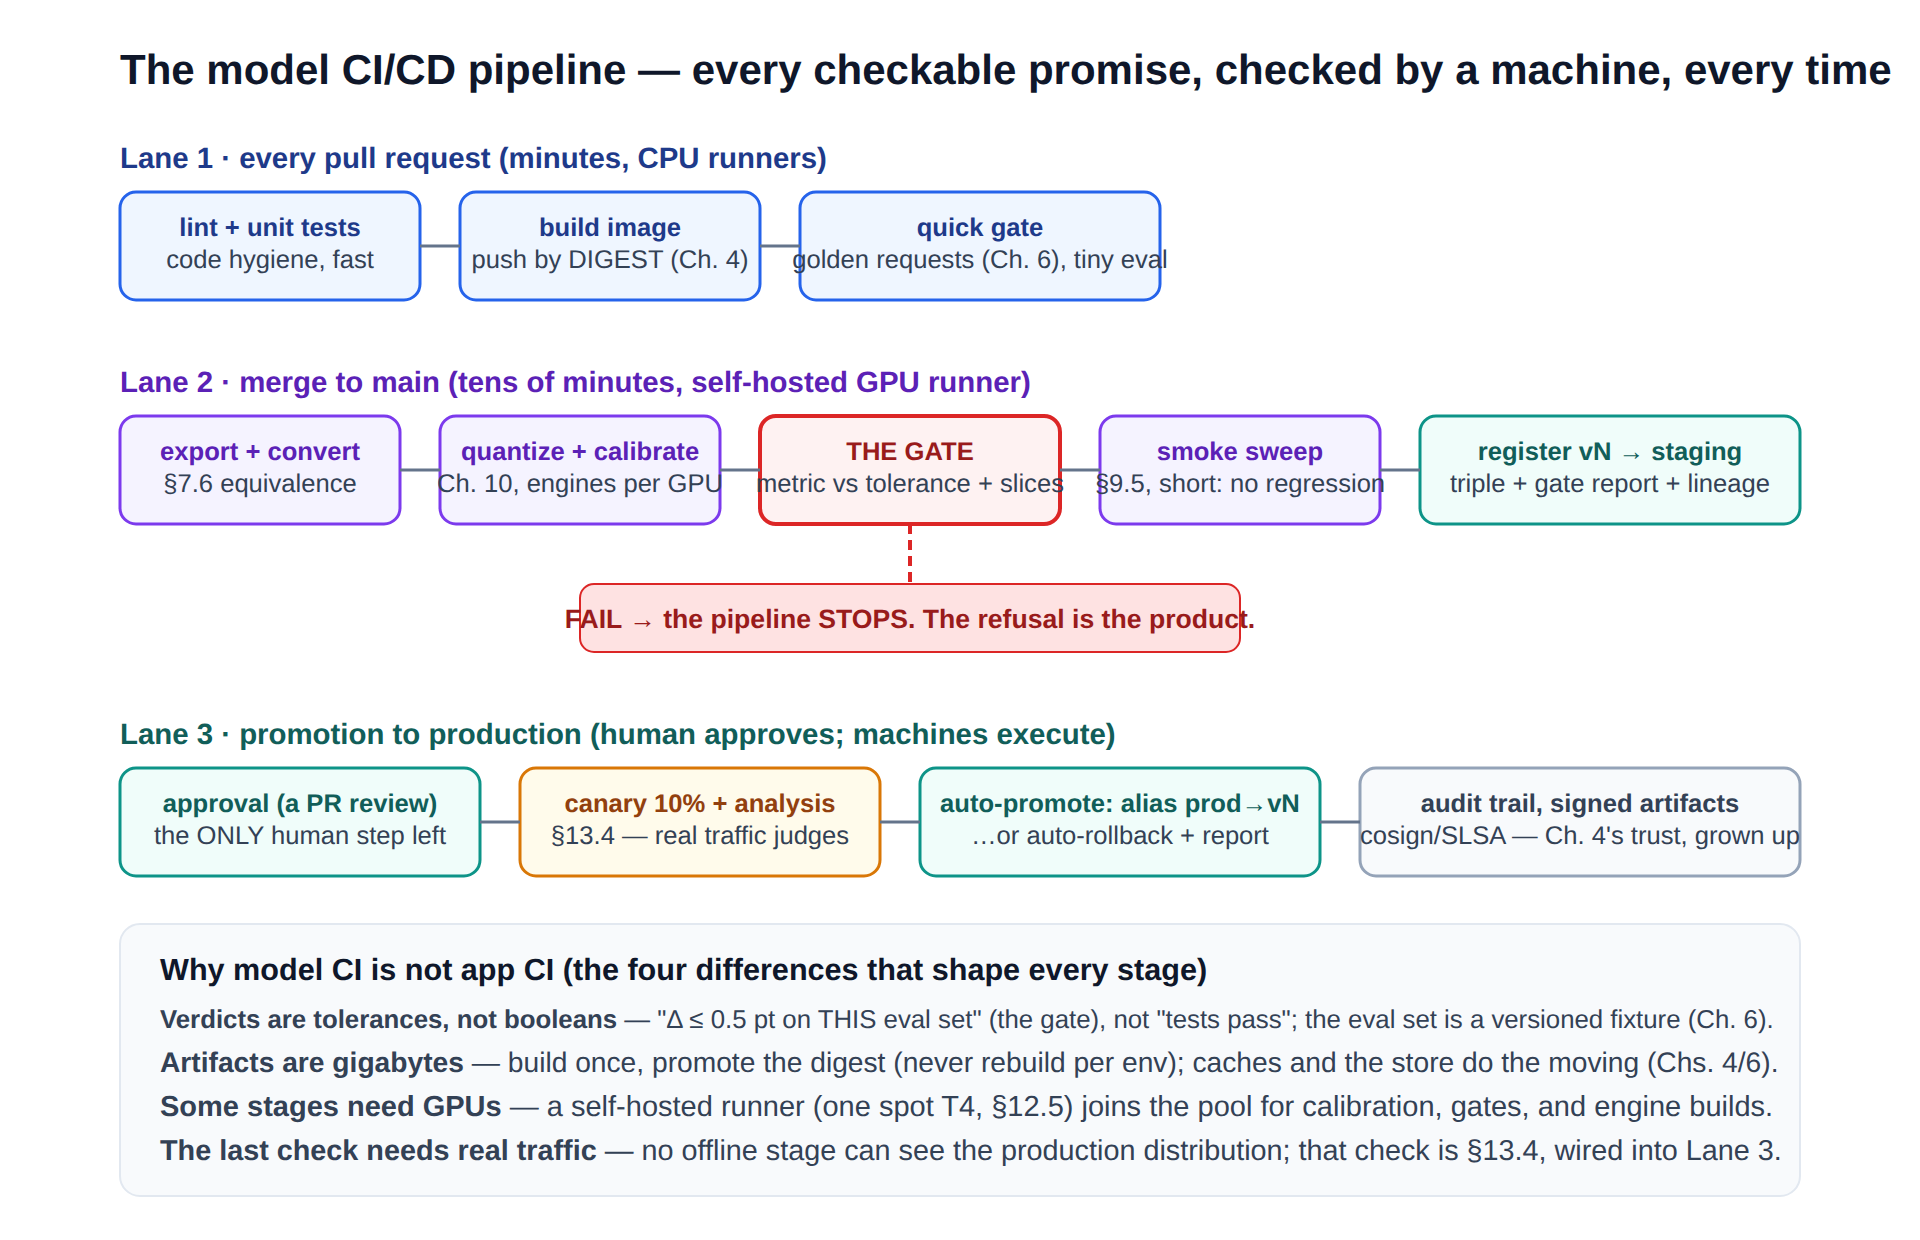
\includegraphics{figures/fig13-3_pipeline.png}}\\[3pt]
  \figcaption{그림 13-3  세 경로. 경로 1은 모든 PR에서 CPU로 빠르게 위생을 검사한다. 경로 2는 모든 병합에서 GPU 러너로 무거운 산출물과 게이트를 처리하고 증거가 있는 등록 릴리스로 끝난다. 경로 3은 사람이 승인하고 카나리가 판정하며 장치가 실행하는 승격이다. 붉은 경로가 제품이다.}
\end{tbbfigure}

\subsection*{모델 CI가 앱 CI와 다른 이유 — 설계를 좌우하는 네 가지 차이}

앱 파이프라인에 모델을 덧붙인 팀은 네 가지 불일치를 발견한다. 그림 13-3의 형태는 각각을 수용한 결과다. \textbf{첫째, 판정은 코드의 불리언이 아니라 데이터에 대한 허용 오차다.} "테스트 통과"는 "\textit{평가 세트 golden-v4에서} Δ ≤ 0.5 pt top-1"이 된다. 따라서 평가 세트 자체도 버전과 다이제스트가 고정된 픽스처다. 시험을 바꾸면 모든 과거 성적의 의미가 조용히 변하므로 제6장에서 이를 저장했다. \textbf{둘째, 산출물은 기가바이트다.} 앱 CI는 환경마다 저렴하게 다시 빌드하지만 모델 CI는 \textbf{한 번 빌드하고 다이제스트를 승격}한다. 같은 바이트가 dev → staging → prod로 흐른다. 제4장의 레지스트리는 빠진 계층만 옮기고 제6장의 저장소는 아무것도 옮기지 않는다. 다른 방식은 "스테이징에서는 동작했다"는 거짓말을 되살린다. \textbf{셋째, 일부 단계에는 실리콘이 필요하다.} 보정, 게이트, 엔진 빌드에는 GPU가 필요하지만 GitHub 호스팅 러너에는 적합한 장치가 없다. 저장소에 등록된 스팟 T4 한 대인 \textbf{자체 호스팅 러너}가 \code{gpu} 태그 작업을 가져간다. 실습 자료 스크립트로 20분이면 설정한다. §12.5의 포트폴리오 사고를 CI에 적용한 것이다. 러너는 중단 가능한 배치 작업으로 스팟의 진정한 용도다. \textbf{넷째, 최종 검사에는 실제 트래픽이 필요하다.} 어떤 오프라인 단계도 프로덕션 분포를 보지 못한다. 따라서 파이프라인의 마지막 단계는 테스트가 아니라 \textit{전략}이다. §13.4의 카나리를 경로 3으로 연결한다.

\begin{terminalbox}
\begin{Verbatim}[breaklines=true,breakanywhere=true,fontsize=\small,formatcom=\color{tbbtermfg},codes=\tbbcodeactive]
# .github/workflows/ci.yaml (condensed - the handout has the full file)
on:
  pull_request:                      # LANE 1: minutes, CPU
  push: {branches: [main]}          # LANE 2: the heavy lane
jobs:
  checks:                           # lane 1
    runs-on: ubuntu-latest
    steps: [lint, unit, docker build --push (by digest),
            quick-gate  # golden requests + 200-sample eval, CPU]
  release-candidate:                # lane 2
    if: github.ref == 'refs/heads/main'
    runs-on: [self-hosted, gpu]     # the spot T4 runner
    steps: [export + equivalence (§7.6),
            quantize + calibrate (Ch. 10),
            gate.py --tol 0.5       # FAIL -> the job fails. loudly.
            smoke-sweep (§9.5, 3 min),
            registry.py register --stage staging  # triple + report]
    permissions: {id-token: write}  # OIDC: no long-lived cloud keys
\end{Verbatim}
\end{terminalbox}
\figcaption{기록 13-3  요약한 워크플로. 경로 1은 몇 분 안에 PR을 정직하게 유지하고, 경로 2는 병합마다 무거운 비용을 한 번 낸 뒤 등록 릴리스로 끝난다. OIDC 줄은 제4장의 인증 질문에 올바르게 답한다. 파이프라인은 몇 분 동안 클라우드 역할을 맡고 유출할 키가 없다.}

\subsection*{중요한 두 실행 — 팀을 바꾸는 문장}

\begin{terminalbox}
\begin{Verbatim}[breaklines=true,breakanywhere=true,fontsize=\small,formatcom=\color{tbbtermfg},codes=\tbbcodeactive]
# run 1: merge 8d31f2 ("switch calib set to 2026-10a")   -- GREEN
  export+equivalence   PASS   max|dz|=3.1e-3, top1-agree 100%   4m
  quantize+calibrate   OK     awq int4, 1.91 GiB                 6m
  gate                 PASS   delta -0.18pt (tol 0.5);
                              worst slice "streetcar" -0.6pt     7m
  smoke sweep          PASS   468 tok/s agg (-2.1% vs base)      3m
  register             OK     chat/v10 -> staging (evidence attached)
  total 22m 14s        bot comment on PR: report + artifact links

# run 2: merge a90c11 ("improve prompt template")        -- RED
  quick-gate           FAIL   golden request 07: expected JSON,
                              got prose; 09: missing citation;
                              12: language mismatch (ko->en)     1m31s
  >> merge blocked. no build, no registry entry, no debate.
# the check that refused has passed 41 times. it is not an opinion.
\end{Verbatim}
\end{terminalbox}
\figcaption{기록 13-4  중요한 두 실행. 녹색은 증거가 있는 레지스트리 항목으로 끝나는 기분 좋은 관료 절차다. 붉은색이 바로 제도다. 91초 안에 이름 붙은 회귀 세 개와 비활성화된 병합 버튼이 나타나 품질 이견이 논쟁으로 번지지 않는다.}

구매한 가치는 붉은 실행이며 문화적 메커니즘도 한 문단을 쓸 만하다. 빠른 게이트가 프롬프트 템플릿 회귀를 잡으면 \textit{병합 버튼이 회색으로 바뀐다.} \textbf{아무도 논쟁하지 않는다.} 거부한 검사는 의견을 가진 동료가 아니라 41번 통과시킨 바로 그 검사다. 파이프라인은 품질 이견을 사람 사이 문제에서 인프라 문제로 바꾼다. 두 규율이 신뢰성을 지킨다. \textbf{건너뛰지도 분기하지도 않는다.} \code{[skip-gate]} 커밋 태그가 생기는 순간 금요일이 돌아온다. 비상 경로는 게이트 생략이 아니라 \textit{더 빠른 카나리}다. \textbf{파이프라인은 자신이 만든 산출물을 먹는다.} 게이트를 거친 것과 배포되는 것은 바이트 단위로 동일해야 한다. 다시 다이제스트다. 검사와 배포 사이에 다시 빌드하면 모든 검사가 무효가 된다. 보안 팀이 언젠가는 보낼 공급망 메모도 미리 반영하자. 산출물 서명(cosign)과 출처 기록(SLSA)은 제4장의 "다이제스트를 신뢰하라"가 성숙한 모습이며 처음부터 경로 2에 넣어야 한다. 지금은 워크플로 두 단계지만 나중에는 발굴 프로젝트가 된다.

실습은 보안 문단 하나를 강제한다. 너무 흔한 실수라 별도 사고 장르가 되었기 때문이다. \textbf{자체 호스팅 러너는 워크플로가 시키는 모든 것을 실행한다.} \textit{공개} 저장소에 붙고 \textit{포크} 풀 리퀘스트로 트리거되는 러너는 GPU, 네트워크 위치, 부주의했다면 클라우드 자격 증명까지 가진 임의 코드 실행 서비스다. 규율은 다음과 같다. 자체 호스팅 러너는 \textbf{비공개 저장소나 포크가 아닌 트리거만} 처리한다. 경로 1에서 포크를 상대하는 검사는 GitHub 호스팅 러너에 남겨 둔다. 러너의 클라우드 역할은 작업에 꼭 필요한 범위로 제한하고 OIDC 신뢰 정책에 저장소와 브랜치를 명시한다. \code{pull\_request\_target}은 문서가 경고하는 대로 위험한 장치로 다룬다. 이국적인 이야기가 아니다. 제2장의 격리 직관을 프로덕션에서 실행할 것을 빌드하는 장치에 적용한 것이다. 그래서 프로덕션보다 덜 민감한 것이 아니라 \textit{더} 민감하다. 파이프라인이 침해되면 이후 모든 녹색 검사는 거짓말이 된다.

\begin{calloutbox}{tbbpurple}{tbbpurplefill}
{\normalsize\bfseries\color{tbbpurple}생각해 보기}\par\vspace{3pt}
\begin{tbbitemize}
  \item 경로 1의 빠른 게이트는 속도를 위해 평가 표본 200개를 쓰고 경로 2의 전체 게이트는 10,000개를 쓴다. 통계적 대가를 계산하라. 실제 회귀가 1.0 pt일 때 각각 어떤 Δ를 신뢰성 있게 감지할 수 있는가? 잡음 ≈ 1/√n이라는 경험 법칙을 사용하라. 경로 1이 정확도 드리프트가 아니라 어떤 버그를 잡기 위해 존재하는지도 설명하라.
  \item 자체 호스팅 GPU 러너는 스팟 인스턴스다. 게이트 중간에 회수되는 실패를 따라가 보자. 워크플로에는 무엇이 표시되는가? 이것이 단지 성가신 일에 그치려면 작업은 어떤 성질을 가져야 하는가? 멱등 단계와 재개 가능한 산출물을 고려하라. CI 러너가 §12.5의 표현대로 스팟의 진정한 용도인 이유도 설명하라.
  \item 팀원이 스윕 처리량에 "req/s@SLO가 >5\% 떨어지면 거부"라는 하드 임곗값 게이트를 적용하자고 한다. 옹호하고 공격하라. 제9장의 어떤 인프라 잡음이 하드 처리량 게이트를 불안정하게 만드는가? 02:00 오경보 없이 신호를 유지할 경고 대 차단, 다시 설정한 기준선 대비 비교의 2단 설계를 제안하라.
  \item "게이트를 절대 건너뛰지 않는다"는 전제에서 팀의 비상 배포 정책을 세 문장으로 작성하라. 비상시 카나리 속도, 승인 정족수, 롤백 사전 스테이징 중 무엇이 바뀌고 무엇은 절대 바뀌지 않는가? Knight에 적용해 정책이 그들을 구했을지 검토하라.
\end{tbbitemize}
\end{calloutbox}

\section{실제 트래픽과 만나기: 롤링, 블루/그린, 카나리, A/B, 섀도}

파이프라인의 마지막 단계는 테스트일 수 없다. 검사할 대상인 \textbf{프로덕션 트래픽}이 오프라인에 존재하지 않기 때문이다. 평가 세트는 지난달 사용자를 비추는 백미러이고 스테이징 클러스터는 축소 모형이다. 오늘 밤의 신조어, 오늘 아침 장애로 생긴 다급한 쿼리, 30k-token 계약서를 붙여 넣는 거대 사용자를 포함한 실제 분포는 정확히 한곳에만 존재한다. 이 절의 각 전략은 새 릴리스의 목줄을 잡은 채 \textit{현실을 만나게} 하는 서로 다른 프로토콜이며, 중요한 규율은 \textbf{서로 다른 질문}에 답한다는 점이다. 유행이 아니라 질문으로 선택한다. 롤링은 \textit{부팅되는가?}, 블루/그린(blue/green)은 \textit{1초 안에 되돌릴 수 있는가?}, 카나리는 \textit{실제 트래픽으로 판단했을 때 고장 났는가?}, A/B는 \textit{사용자가 판단할 때 더 나은가?}, 섀도는 누구도 위험을 감수하기 전에 \textit{무엇을 했을 것인가?}를 묻는다.

\begin{tbbfigure}
  \adjustbox{max width=0.94\linewidth,max totalheight=0.46\textheight}{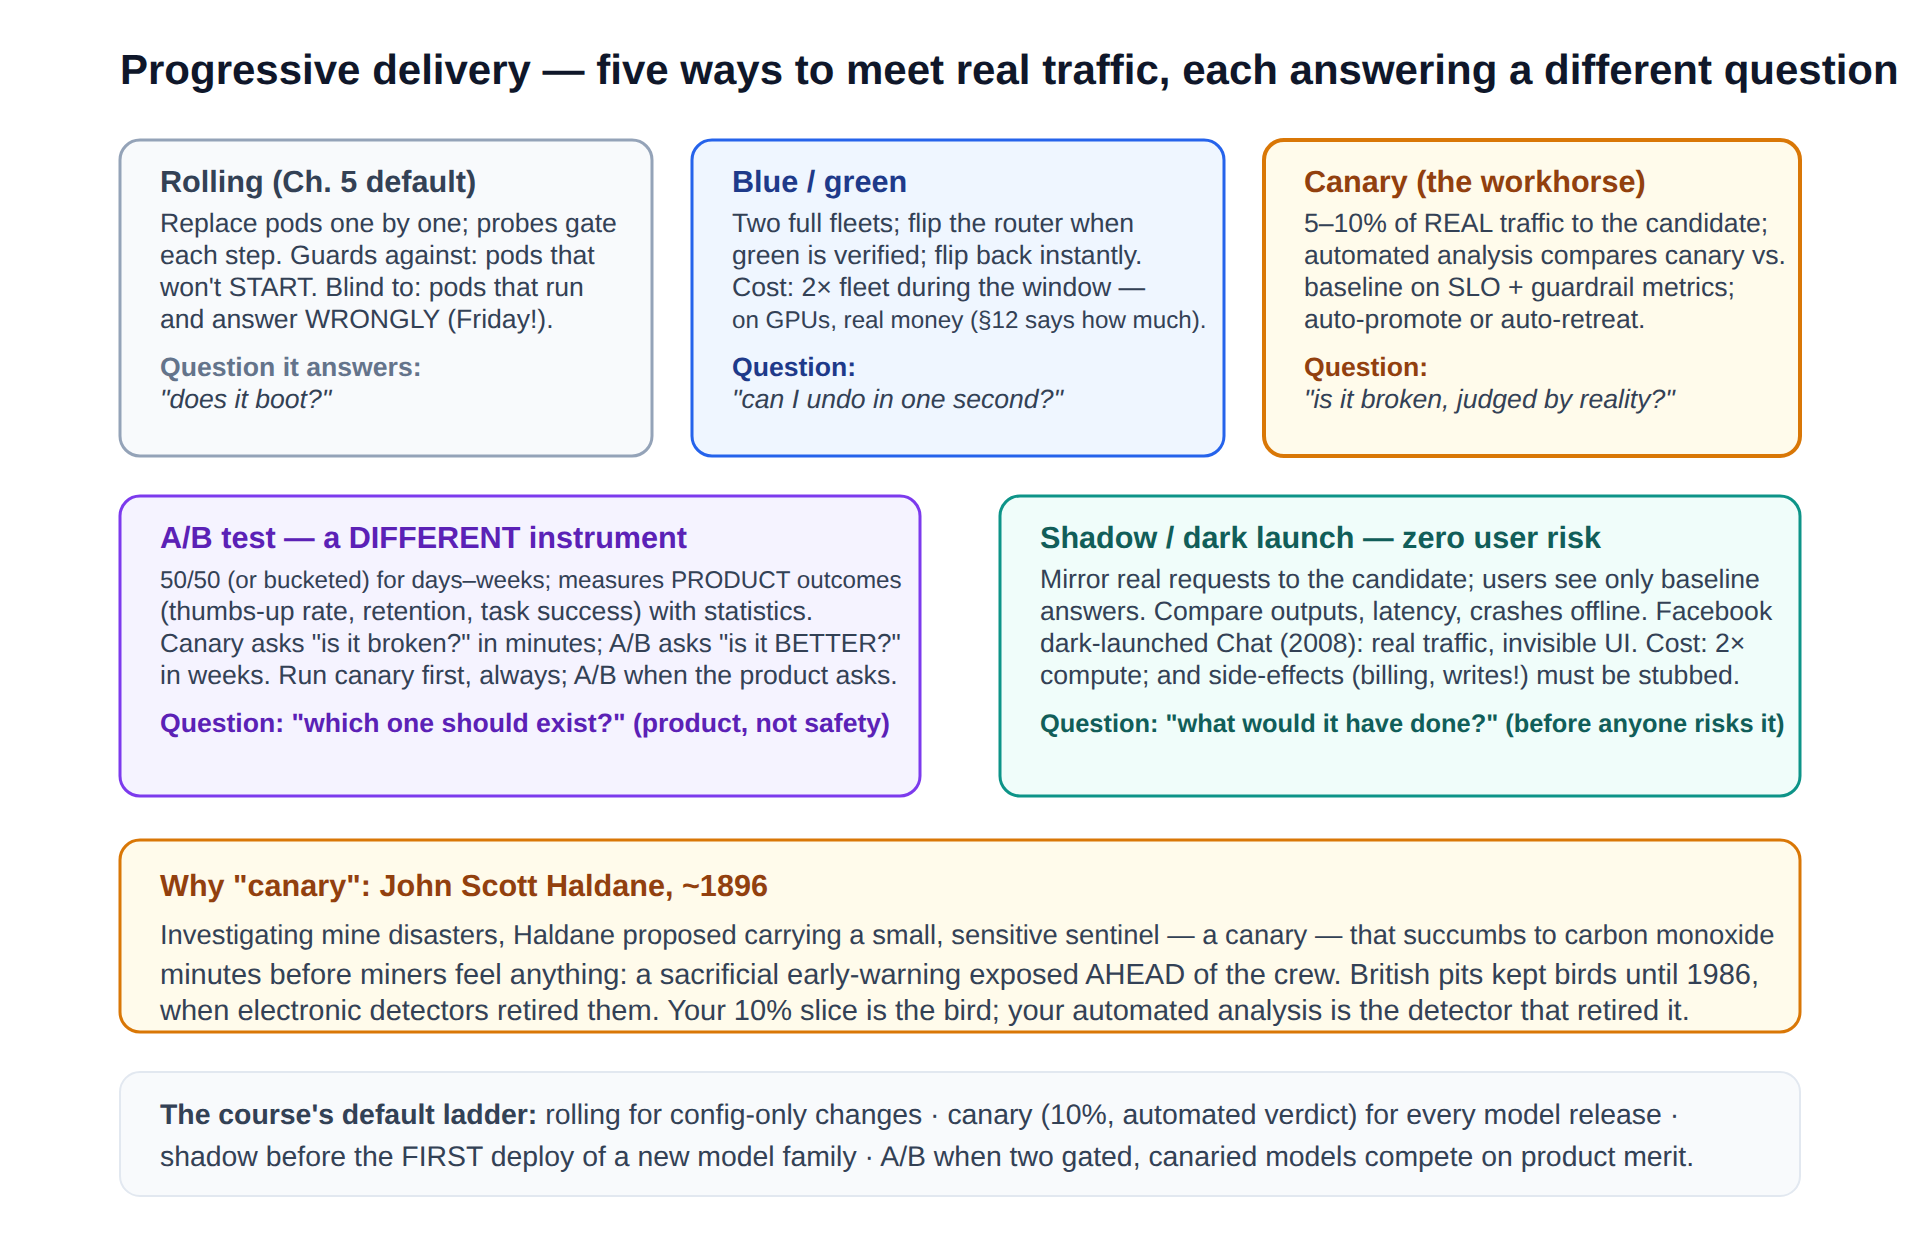
\includegraphics{figures/fig13-4_strategies.png}}\\[3pt]
  \figcaption{그림 13-4  다섯 전략과 다섯 질문. 롤링은 시작을 보호하고, 블루/그린은 2× 플릿 비용으로 즉시 되돌리기를 사며, 카나리는 실제 트래픽을 판정하는 핵심 도구다. A/B는 안전이 아니라 제품 도구이고 섀도는 사용자 위험 없이 연습한다. 아래에는 Haldane의 새와 이를 은퇴시킨 감지기가 있다.}
\end{tbbfigure}

\subsection*{롤링과 블루/그린 — 물려받은 두 단}

\textbf{롤링}은 제5장부터 사용했다. 파드를 몇 개씩 교체하고 준비 상태 프로브가 각각의 입장을 허용한다. 정확히 무엇을 보호하는지 알아야 한다. \textit{시작하지 못하거나 프로브에 실패하는 파드}를 막는다. 반대로 무엇을 보지 못하는지도 알아야 한다. 금요일 파드는 아름답게 시작했고 따뜻함을 확인하는 프로브를 통과했으며 완벽한 상태로 짧은 답을 서빙했다. 롤링만으로 충분한 경우는 의존성 업데이트나 자원 조정처럼 실패 유형이 시작 자체인 변경뿐이다. 모델 릴리스에서는 더 영리한 전략이 올라타는 \textit{기반}이다. \textbf{블루/그린}은 전체 플릿 두 개를 실행한다. 블루가 서빙하고 그린은 후보를 올린 채 쉬며, 그린을 스모크 테스트와 따뜻한 캐시로 검증한 뒤 라우터를 전환한다. 후회하면 몇 초 만에 다시 전환한다. GPU 플릿에서의 정직한 문제는 제12장의 계산이다. 둘째 플릿은 둘째 청구서다. 릴리스 창마다 교재 플릿에 \textasciitilde{} \$1,500/mo가 들며 몇 분 동안은 견딜 수 있지만 습관이 되면 터무니없다. 전환 전 검증도 여전히 \textit{합성} 트래픽이므로 롤링처럼 금요일 유형 버그를 보지 못한다. 블루/그린은 엔진 업그레이드, CUDA 업데이트처럼 즉시 되돌리기가 필요한 \textit{설정/인프라} 릴리스에서 빛난다. 라우터 전환 메커니즘은 우연이 아니라 카나리가 더 세밀하게 재사용하는 힘이다.

\subsection*{카나리 — Haldane의 새와 새를 은퇴시킨 감지기}

핵심 도구의 어원은 비유 자체가 시스템을 지탱하므로 살펴볼 가치가 있다. 1890년대 광산 폭발을 조사한 생리학자 \textbf{John Scott Haldane}은 작업자가 작고 온혈인 보초인 카나리를 데리고 다니자고 제안했다. 대사가 더 빨라 광부가 아무것도 느끼기 \textit{몇 분 전}에 일산화탄소에 쓰러졌다. 작업자 \textbf{앞에 노출}한 민감하고 희생적인 감지기로, 새가 노래를 멈추고 휘청이는 모습을 저렴하게 관찰하고 밖으로 나가는 저렴한 조치를 취할 수 있었다. 영국 광산은 전자 감지기가 마침내 은퇴시킨 \textbf{1986년}까지 새를 데리고 다녔다. 모든 조항을 대응시켜 보자. \textbf{카나리 릴리스}는 실제 트래픽의 5–10\%를 받아 새가 실제 공기를 마시게 하고, 90\%는 기존 릴리스에 두어 작업자가 입구에서 기다리게 한다. \textbf{자동 분석}이 카나리를 지켜본다. 1911년보다 발전한 전자 감지기라 누구도 새를 봐야 한다는 사실을 기억할 필요가 없다. 나쁜 판정은 몇 초 안에 밖으로 나가는 \textbf{자동 후퇴}를 일으킨다. 이 교재 영역에서는 세 설계 선택이 성공을 좌우한다. \textit{요청이 아니라 세션으로 분할}한다. 제11장의 대화는 한쪽에 온전히 살아야 한다. 대화 ID의 일관된 해시로 §11.5의 어피니티 메커니즘을 다른 용도에 쓴다. 그렇지 않으면 사용자는 인격이 깜박이는 것을 보고 메트릭은 뒤섞인 것을 비교한다. \textit{카나리와 기준선을 동시에 비교}하고 어제와 비교하지 않는다. 트래픽 자체에 제12장의 일중 성격이 있어 같은 시각의 대조군만 릴리스를 분리한다. \textit{SLO뿐 아니라 가드레일을 관찰}해야 한다. 여기서 금요일 버그가 수업료를 낸다.

\begin{tbbfigure}
  \adjustbox{max width=0.94\linewidth,max totalheight=0.46\textheight}{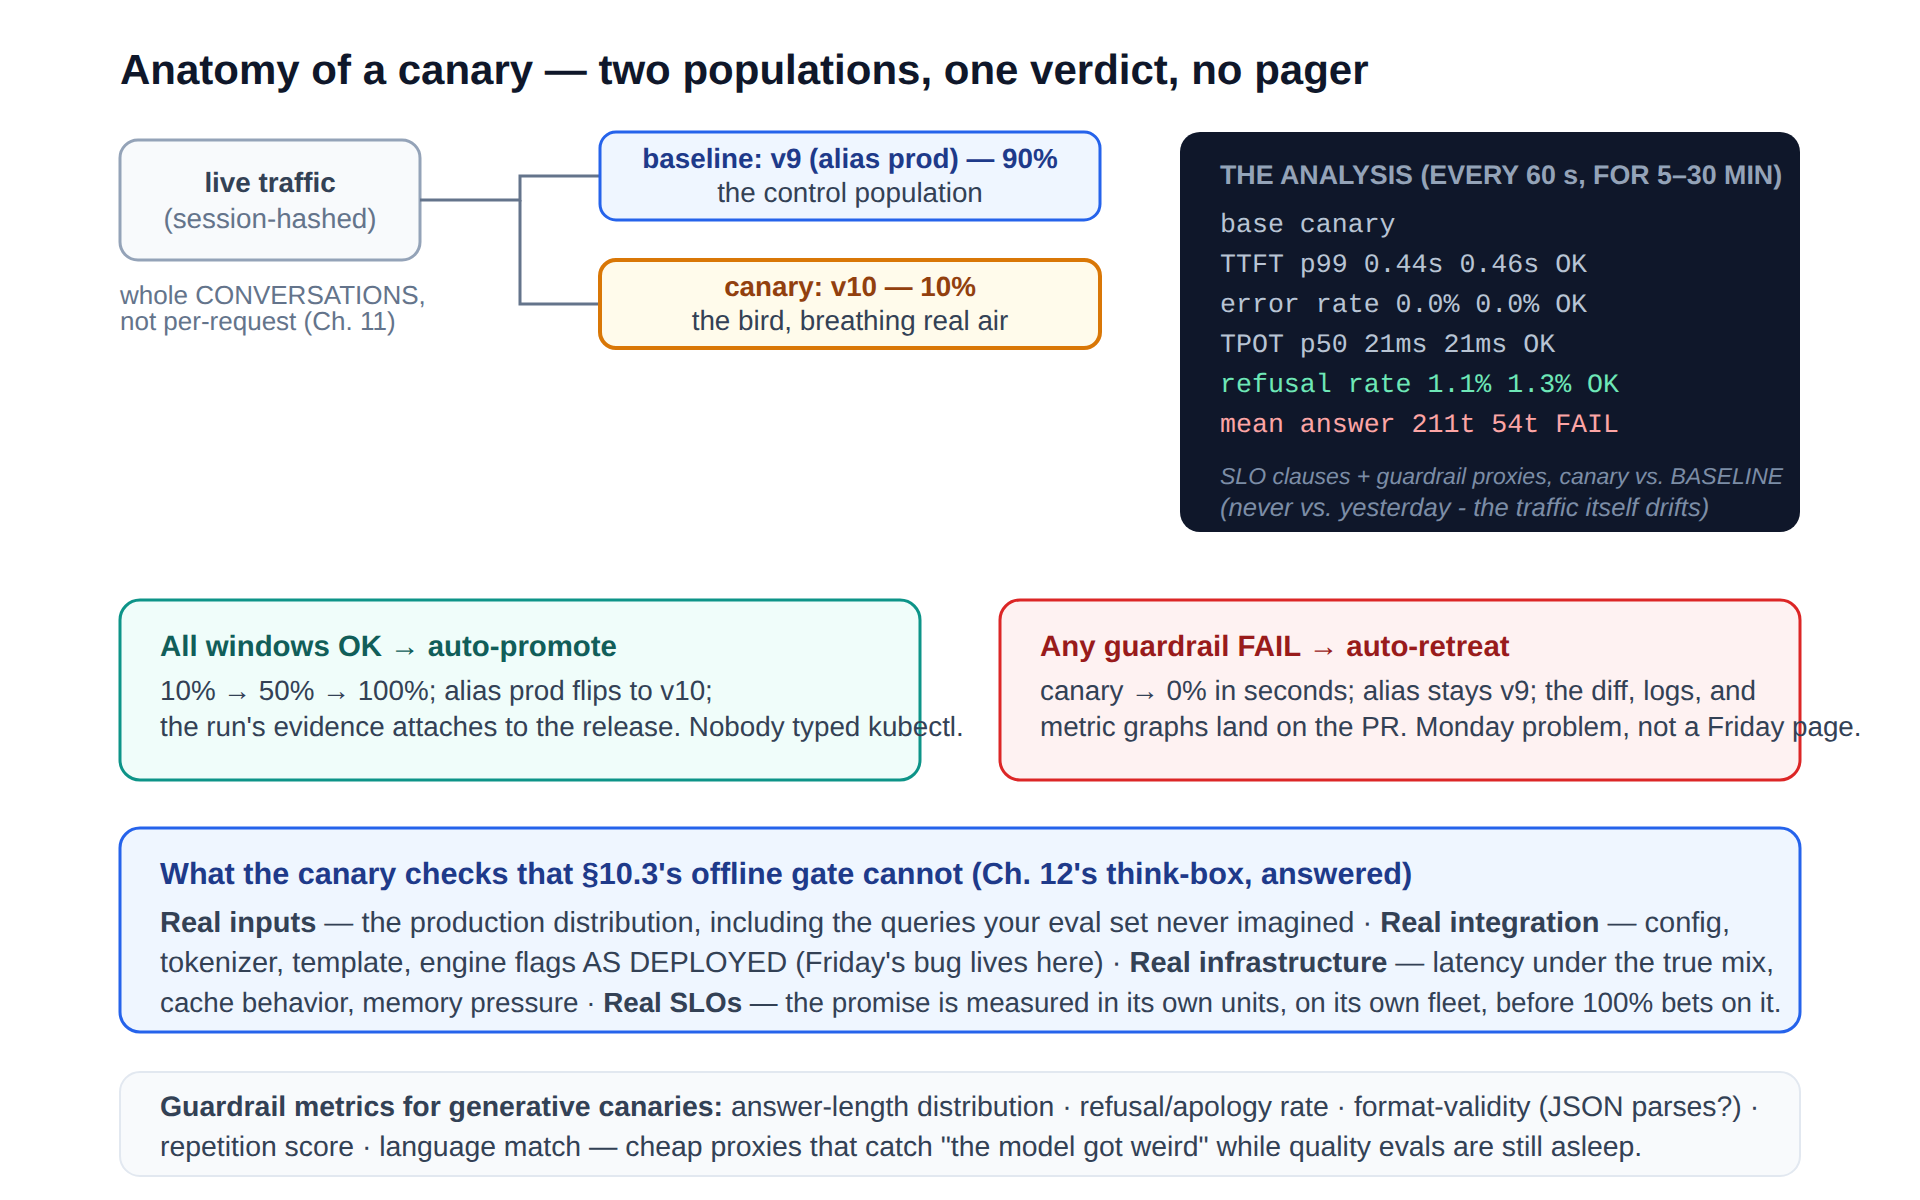
\includegraphics{figures/fig13-5_canary.png}}\\[3pt]
  \figcaption{그림 13-5  카나리의 구조. 세션 해시 분할, 동시 기준선, SLO 조항과 가드레일 프록시를 확인하는 60초 분석 루프, 두 자동 출구로 구성된다. FAIL 행은 금요일 버그를 10\% 노출에서 5분 안에 잡은 모습이다.}
\end{tbbfigure}

\textbf{가드레일 메트릭}은 생성 시대가 카나리 전통에 더한 요소다. §13.1의 생각해 볼 문제에서 이미 발명했다. 진짜 품질 평가가 아직 잠든 동안 \textit{"모델이 이상해졌다"}를 잡는 저렴하고 모델에 구애받지 않는 프록시다. 교재에서 사용하는 집합은 모두 60초 루프에서 로그로 계산할 수 있다. \textbf{답변 길이 분포}는 금요일의 211 → 54 tokens를 한 창 안에서 외친다. \textbf{거부/사과 비율}은 과도한 정렬 회귀를 잡고, \textbf{형식 유효성}은 JSON이 파싱되는지 인용이 해석되는지 확인한다. \textbf{반복 점수}와 \textbf{언어 일치}도 본다. 한국어 질문에는 한국어 답이 나와야 한다. 어느 것도 "좋음"을 측정하지 않고 모두 \textit{동작의 동일성}을 측정한다. 바로 이것이 배포의 귀무가설이다. 제11장의 TTFT/TPOT/오류라는 SLO 조항이 시스템을 지키고 가드레일은 \textit{동작}을 지킨다. 더 미묘한 것은 A/B를 기다린다. 판정 논리는 의도적으로 단순하게 둔다. 고정 창, 기준선 대비 명시적 임곗값, 하나라도 실패하면 후퇴한다. 원시 Deployment에서는 제5장의 더 읽을거리에 등장한 Argo Rollouts가 단계별 가중치와 Prometheus 분석을 자동화한다. InferenceService에서는 제12장이 남긴 KServe의 \code{canaryTrafficPercent}가 이를 수행한다. 실습은 마법이 없음을 보여 주려고 후자를 40줄 루프로 제어한다.

\begin{terminalbox}
\begin{Verbatim}[breaklines=true,breakanywhere=true,fontsize=\small,formatcom=\color{tbbtermfg},codes=\tbbcodeactive]
$ gh workflow run deploy.yaml -f version=v10      # lane 3, replayed
14:00:12  canary: chat canaryTrafficPercent 0 -> 10 (session-hashed)
14:01:12  window 1/5:  TTFT p99 0.46s vs 0.44s OK | err 0.0% OK
          | ans-len 208t vs 211t OK | refusal 1.2% vs 1.1% OK
14:02:12  window 2/5:  all OK
14:03:12  window 3/5:  ans-len 55t vs 210t
          guardrail: |delta| 74% > 30%  -> FAIL
14:03:14  verdict: RETREAT. canary 10% -> 0%. alias prod stays v9.
14:03:20  posted to PR #241: verdict, metric graphs, sample diffs
          (12 canary answers, all ending mid-sentence at 54 tokens)
# exposure: ~10% of users for 3m02s = 0.3 bad user-minutes.
# friday, replayed with institutions: the bird went quiet,
# the detector noticed, the crew never entered the mine.
\end{Verbatim}
\end{terminalbox}
\figcaption{기록 13-5  금요일 버그 대 카나리. 세 창에서 가드레일 하나가 작동하고 자동 후퇴했으며 수정이 일어날 곳에 증거를 기록했다. 사람의 개입이 필요하지 않아 아무도 호출받지 않았다. 사고 전체가 PR 댓글 하나다.}

\subsection*{얼마나 길어야 충분한가 — 냅킨 위의 카나리 통계}

창 길이는 속설이 아니라 머릿속으로 계산할 수 있는 표본 크기 문제다. 교재 플릿은 피크에 \textasciitilde{}23 turn-arrivals/s를 흡수하므로(§11.2) 10\% 카나리는 \textbf{\textasciitilde{}2.3 requests/s ≈ 5분에 답변 690개}를 본다. 690개 표본이 감지할 수 있는 것은 효과 크기에 전적으로 달려 있다. 답변 길이가 211 → 54 tokens로 74\% 떨어지고 분포 폭이 \textasciitilde{}±30\%인 금요일의 절벽은 \textit{첫} 60초 창 안에서도 명백하다. 절벽에는 수십 개 표본이면 충분하므로 기록 13-5의 판정은 여유 있게 세 번째 창에 나온다. 하지만 형식 유효성이 97\%에서 3\% 떨어지는 \textit{미묘한} 회귀는 잡음과 구분하기 위해 각 집단에 수천 개 표본이 필요하다. 이항 경험 법칙은 감지 가능한 Δ ≈ 2√(p(1−p)/n)이며 n = 690에서는 잘해야 약 ±1.3 percentage points다. 기억할 설계 태도는 \textbf{카나리는 기울기가 아니라 절벽을 잡는다}는 것이다. 충돌, SLO 위반, 가드레일 급변이라는 절벽 유형에 짧은 체류와 단단한 임곗값을 설정한다. 기울기는 이를 위해 만든 도구에 맡긴다. 제14장의 드리프트 모니터는 몇 주의 프로덕션 데이터를 보고, §13.4의 A/B는 균형 잡힌 집단과 사전 등록한 검정력을 사용한다. 단계 증가 일정도 노출 제어와 같은 논리를 인코딩한다. 1\% → 10\% → 50\% → 100\%로 각 단계에서 머무르면 가장 저렴한 절벽은 1\%에서 잡고, 충돌에는 \textasciitilde{}10개 표본이면 충분하다. 가드레일 절벽은 10\%에서 잡고 "더 지켜보자"는 롱테일은 마지막 체류로 제한한다. 각 단계는 사용자 노출로 감지력을 구매하며, 일정을 적어 두면 판단이 설정 필드가 된다.

\subsection*{A/B와 섀도 — 나머지 두 질문}

\textbf{A/B 테스트}는 카나리의 트래픽 분할 배관만 공유하고 \textit{나머지는 전혀 공유하지 않는다.} 둘을 혼동하는 것이 이 절의 고전적 오류다. 카나리는 몇 분에서 몇 시간 동안 작은 비율을 노출하고 "같이 동작한다"는 귀무가설을 자동 판정하는 \textbf{안전} 도구다. A/B는 며칠에서 몇 주 동안 크고 균형 잡힌 버킷(흔히 50/50)을 두고 "v10의 답이 \textit{더 낫다}"는 가설을 실제 통계로 검증하는 \textbf{제품} 도구다. 사전 등록한 메트릭, 검정력 분석, 신규성 효과를 기다리는 인내와 함께 좋아요 비율, 작업 완료, 유지율 같은 제품 결과를 측정한다. LLM 제품에서 A/B는 품질 주장을 정직하게 시험하는 곳이다. 실제 세션 승률이 어떤 오프라인 벤치마크보다 낫다. 하지만 후보가 이미 게이트와 카나리를 통과했다고 \textit{전제}한다. 안전한 모델 두 개 중 무엇이 존재해야 하는지 배우려고 A/B를 하지, 어느 것이 고장인지 찾으려고 하지 않는다. \textbf{섀도(다크 론치)}는 사용자 위험 0으로 스펙트럼을 완성한다. 실제 트래픽 복사본을 후보에 미러링하고 사용자는 기존 릴리스의 답만 본다. 섀도의 동작을 오프라인에서 비교해 노출 전에 충돌, 실제 혼합에서의 지연 시간, 출력 드리프트를 확인한다. Facebook의 유명한 2008년 Chat \textbf{다크 론치(dark launch)}는 이를 규모 있게 실행했다. 몇 주 동안 UI 없이 페이지가 조용히 연결을 열고 실제 트래픽 형태로 메시지 경로를 모사해 출시일 부하는 백엔드에 이미 익숙했다. 비용도 실제다. 미러링한 부분에 추론 연산이 \textasciitilde{}2× 들며 제12장의 가격으로 트래픽 10\% 섀도는 10시간마다 레플리카 시간 하나 정도다. \textbf{부작용은 스텁 처리}해야 한다. 결제에 쓰고 이메일을 보내거나 공유 캐시의 KV를 변경하는 섀도는 연습이 아니라 둘째 프로덕션이다. 첫 vLLM 배포, 새 기반 모델, 엔진 메이저 버전처럼 \textit{계열 경계}에서 섀도는 비용만큼 가치가 있다. 카나리 10\%도 진정으로 알 수 없는 동작에 실제 사용자 10\%를 노출하기 때문이다.

교재의 기본 사다리를 그림 13-4 아래 띠에 따라 한 줄씩 정리하자. 실패가 시작 형태인 코드/설정 변경에는 \textbf{롤링}만 쓴다. 예외 없이 \textit{모든} 모델 릴리스에는 \textbf{자동 분석이 있는 카나리}를 적용한다. 이 교재 전체에서 절감한 피해 사용자-분당 가장 저렴한 제도다. 릴리스가 계열 경계를 넘으면 \textbf{섀도를 먼저} 쓰고, 게이트와 카나리를 통과한 후보 두 개가 성능으로 겨룰 때 \textbf{A/B}를 쓴다. 압박에서도 사다리가 동작하게 하는 상위 규칙은 \textbf{전략이 영웅적 선택이 아니라 파이프라인 단계}라는 것이다. 화요일 오후든 금요일 18:07이든 경로 3은 같은 YAML을 실행한다. 바로 그것이 목적이다.

\begin{calloutbox}{tbbpurple}{tbbpurplefill}
{\normalsize\bfseries\color{tbbpurple}생각해 보기}\par\vspace{3pt}
\begin{tbbitemize}
  \item 카나리는 통과했지만 일주일 뒤 사용자가 불만을 제기한다. 30분 카나리가 구조적으로 잡을 수 없는 세 실패 유형인 느리게 진행되는 품질 드리프트, 저빈도 슬라이스, 신규성 효과를 나열하고 각각을 잡는 §13.4 또는 제14장의 도구를 제시하라.
  \item 세션 해시는 대화의 10\%를 카나리로 보낸다. 하루 대화가 200개인 헤비 사용자는 "항상 이상한 버전이 걸린다"고 불평한다. 세션별 해시와 사용자별 해시에서 확률을 계산하고 분할 키를 다시 설계하라. 수정이 분석의 표본 독립성에 어떤 비용을 부과하는가?
  \item 교재 프로젝트의 섀도 하네스를 자세히 설계하라. 트래픽은 어디에서 분기하는가(LB, 사이드카, 로그의 비동기 탭)? 무엇을 스텁 처리하고 무엇을 비교하며, "카나리 준비 완료"를 결정하는 단 하나의 수치는 무엇인가? §12 비용 항목도 포함하라.
  \item PM은 "작은 프롬프트 수정"에 카나리를 건너뛰고 싶어 한다. "작은 설정" 변경인 사례 13-A, 가드레일 표, 한계 비용이 거의 0인 카나리 비용을 이용해 두 문장으로 답하라. 파이프라인은 어차피 카나리를 실행한다. 카나리를 생략해도 실제로 정당한 변경 클래스 하나도 제시하라. 힌트는 §13.4의 첫 단이다.
\end{tbbitemize}
\end{calloutbox}

\section{관리형 엔드포인트: 완성된 오퍼레이터 사다리}

이 장에서 구축한 모든 것을 누군가는 판매한다. AWS의 \textbf{SageMaker 엔드포인트}와 GCP의 \textbf{Vertex AI 엔드포인트}, 그리고 모든 클라우드의 유사 서비스는 제12장에서 시작한 오퍼레이터 사다리의 마지막 단이다. 직접 구축 방식에서는 사용자가 모든 것을 운영하고, 플랫폼에서는 KServe 오퍼레이터가 \textit{사용자} 클러스터의 서빙 배관을 운영하며, \textbf{관리형}에서는 공급자의 오퍼레이터와 클러스터와 호출기를 쓴다. 모델 산출물을 업로드하고 인스턴스 유형을 고르면 공급자가 제5–12장에서 구축한 것을 만들어 낸다. 프로비저닝, 오토스케일링, 상태 기반 라우팅, 로깅, 패칭에 더해 이 장과 관련된 \textbf{프로덕션 변형 / 트래픽 분할}을 제공한다. 카나리가 필드가 되어 SageMaker는 \code{InitialVariantWeight}, Vertex는 \code{trafficSplit \{v9: 90, v10: 10\}}을 쓴다. 승인 워크플로가 있는 \textbf{모델 레지스트리}와 경보 시 자동 롤백하는 \textbf{배포 가드레일}, 즉 §13.4의 분석을 체크박스로 판매한다. 용어가 일대일로 대응하므로 이 절은 짧다. 조절점을 직접 만들었으니 각 조절점의 역할을 이미 안다.

\begin{tbbfigure}
  \adjustbox{max width=0.94\linewidth,max totalheight=0.46\textheight}{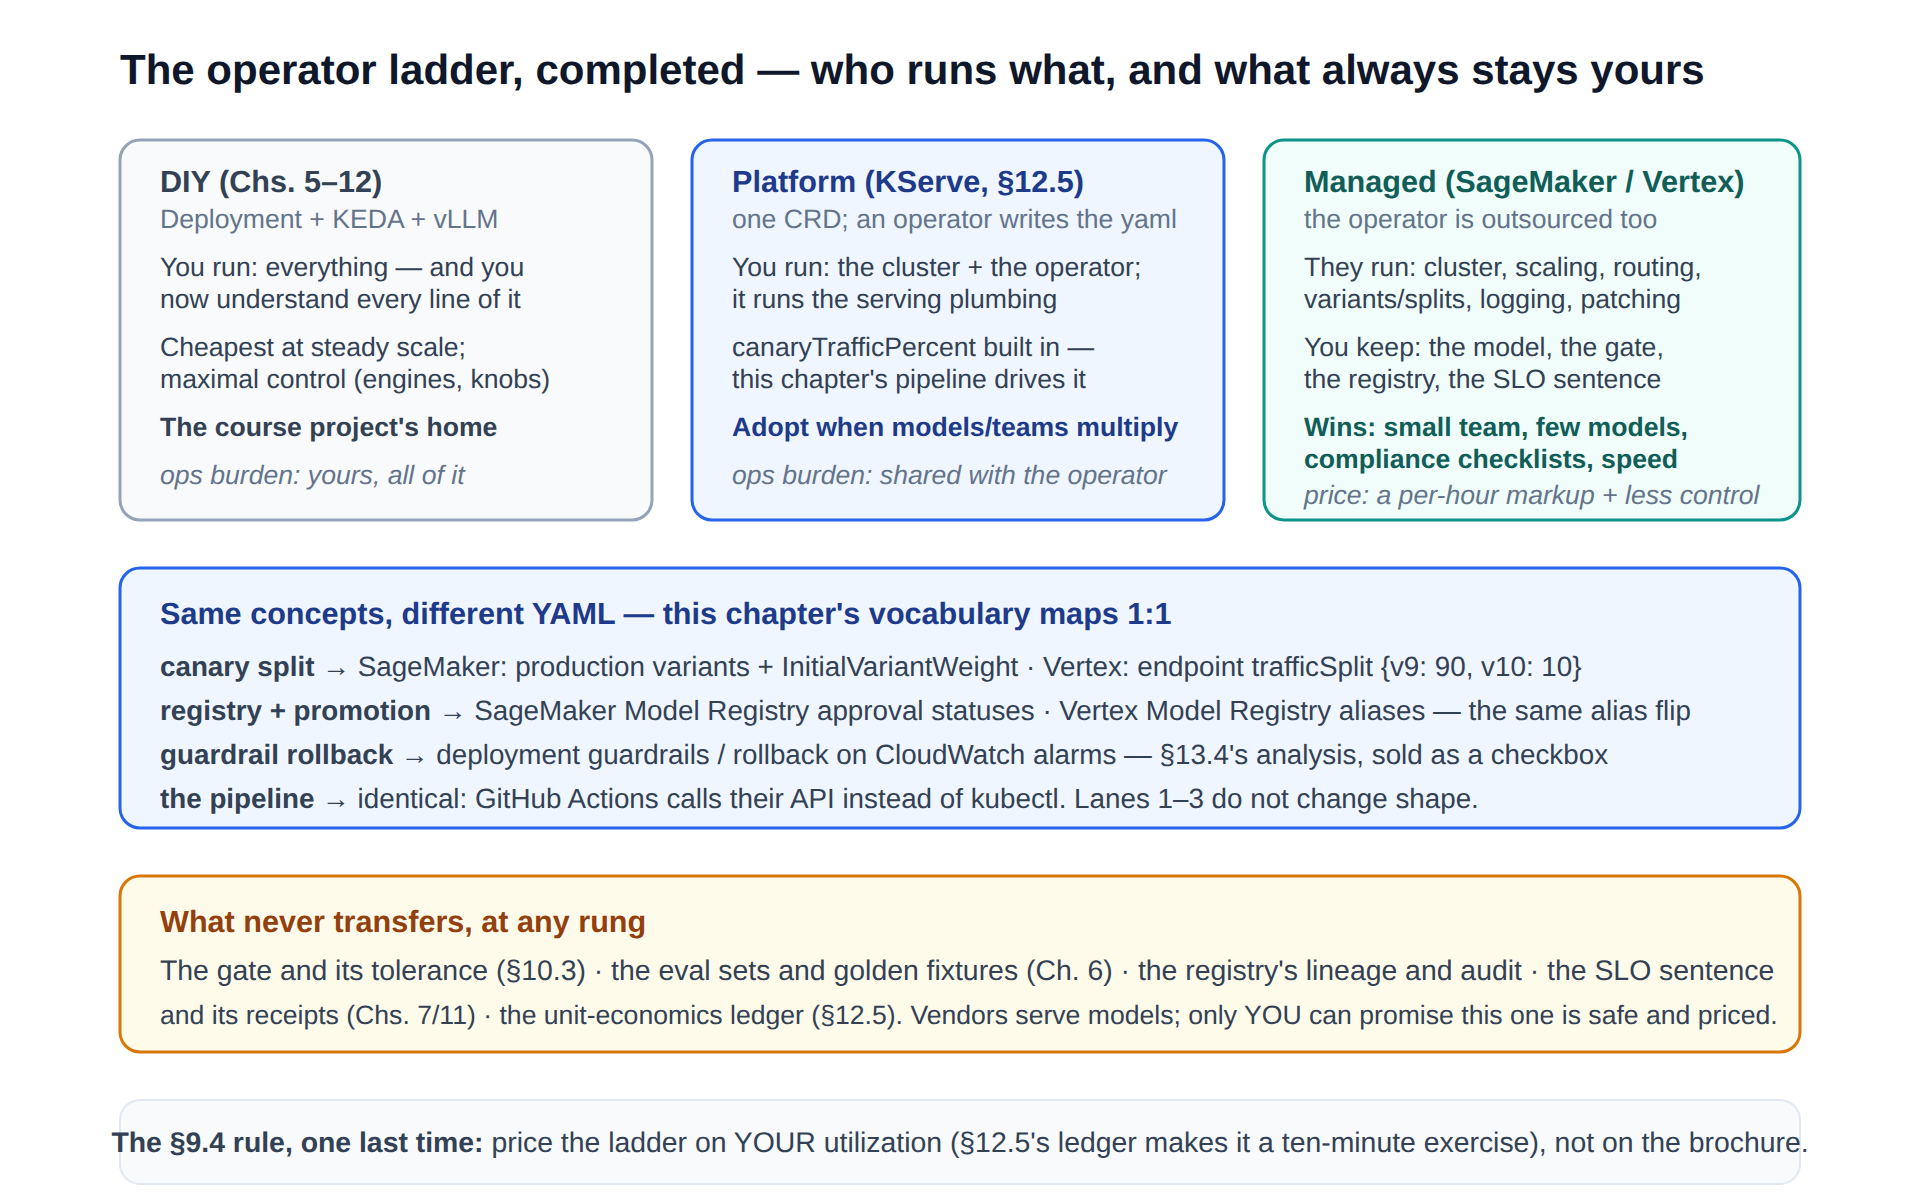
\includegraphics{figures/fig13-6_managed.png}}\\[3pt]
  \figcaption{그림 13-6  사다리의 마지막 단. 관리형 엔드포인트는 배관을 운영하고 이 장의 전략을 필드로 판매한다. 하지만 게이트, 평가 세트, 레지스트리 계보, SLO 문장, 단위 경제성 원장은 어느 단에서도 영원히 사용자 몫이다.}
\end{tbbfigure}

이제 가진 도구로 정직한 절충의 가격을 매겨 보자. \textbf{얻는 것}은 운영 팀이 0명이어도 오늘 오후에 프로덕션 모델을 실행하고, 규정 준수 점검표가 공급자 인증을 물려받으며, 차별화되지 않는 무거운 작업인 노드 풀, 드라이버, CVE 패칭, §12.3의 콜드 스타트 엔지니어링이 다른 사람의 3분기 일이 된다는 점이다. \textbf{지불하는 것}은 원시 VM보다 인스턴스 시간당 붙는 \textbf{마진}이다. 흔히 수십 퍼센트이므로 어느 방향의 주장도 믿기 전에 자신의 사용률로 §12.5 원장을 계산해야 한다. 서빙 스택 제어도 줄어든다. 엔진 버전, §9/§11 조절점, 사용자 정의 커널이 공급자 일정에 맞춰 도착하고, 자신의 정책이 아니라 공급자의 콜드 스타트와 0으로 스케일링 정책을 따른다. 이그레스, IAM 연결망, 재학습 역량의 퇴화라는 중력도 생긴다. 결정은 정장을 입은 제9장의 벤치마크 규칙이다. \textit{홍보 자료가 아니라 자신의 사용률과 팀을 기준으로 사다리 가격을 계산하라.} 작은 팀 + 적은 모델 + 스파이크 트래픽은 관리형 쪽이고, 안정적 규모 + 비용 압박 + 엔진 수준 튜닝은 아래 단 쪽이다. 이 교재의 프로젝트는 의도적으로 후자다. 어느 단에서도 절대 이전되지 않는 자산이 있다. \textbf{게이트와 허용 오차, 평가 픽스처, 레지스트리의 계보와 감사, 근거가 있는 SLO 문장, \$/M-token 원장}이다. 공급자는 모델을 서빙하지만 \textit{이} 모델이 안전하고 가격이 적절하며 정직하게 측정되었다고 약속할 수 있는 것은 사용자뿐이다. 눈치챘겠지만 이 목록이 바로 이 교재다.

"원장을 계산하라"는 과제로만 남기지 않고 한 번 보여 줄 가치가 있다. §12.5의 계산으로 교재 플릿을 관리형 단에서 다시 가격 책정하자. L4급 인스턴스에 대표적인 \textbf{35\% 마진}이 붙고 공급자 오토스케일링이 같은 61 rep-h/day 계단을 따른다고 가정한다. 공급자의 0으로 스케일링 정책이 바닥 2개 논리를 이기는 경우는 드물어 그대로 유지한다. 61 × 31 × (\$0.80 × 1.35) ≈ \textbf{\$2,042/mo}이며 자체 호스팅 \$1,513보다 \$529/mo 비싸다. 관리형 단에는 약정을 적용할 수 있지만 사용자의 스팟 버스트 기법은 쓸 수 없어 현실적인 격차는 \textbf{\textasciitilde{}\$1,100/mo 대 \$877} 쪽으로 벌어진다. 프리미엄이 사는 것을 유일하게 정직한 단위로 가격을 매기면 §12.2–12.3을 구축하지 않고 §13.4를 체크박스로 사용하며 패칭 반복 작업을 피하는 \textbf{분기당 엔지니어 약 1주}다. 모델 세 개를 가진 2인 팀에는 이 거래가 흔히 \textit{옳다.} 인기 모델 하나에 엔진 수준 튜닝을 하고 모든 조절점을 이제 소유한 이 교재 프로젝트에는 그렇지 않다. 중요한 것은 판정 자체가 아니라 홍보 자료 없이 계산 네 줄로 판정했다는 점이다. 14주간 측정한 수치는 바로 이를 위한 것이다.

\begin{calloutbox}{tbbpurple}{tbbpurplefill}
{\normalsize\bfseries\color{tbbpurple}생각해 보기}\par\vspace{3pt}
\begin{tbbitemize}
  \item 롱테일에 0으로 스케일링을 포함하고 인스턴스 마진 35\%인 관리형 엔드포인트에서 기록 12-6 원장을 다시 작성하라. 어느 플릿 크기에서 마진이 연간 SRE 한 달을 넘으며, GPU 가격이 아니라 이것이 실제 손익분기 질문인 이유는 무엇인가?
  \item 규제를 받는 고객은 "하이퍼바이저 아래에 공유 인프라가 없어야 한다"고 요구한다. 제2장의 격리 용어인 패스스루, MIG, 멀티테넌트 컨트롤 플레인으로 사다리의 각 단을 요구사항과 비교하라. 어느 단이 살아남고 비용은 얼마인가?
  \item 현재 파이프라인 경로 1–3은 kubectl을 대상으로 한다. 배포 대상이 Vertex 엔드포인트로 바뀌면 정확히 어느 단계가 바뀌는지 나열하라. 힌트: 경로 3의 동사만 바뀐다. 검사한 것을 무효로 만들지 않으려면 삼중항, 게이트 보고서, 레지스트리 항목 중 무엇이 바뀌지 않아야 하는가?
  \item 관리형 가드레일은 인프라 메트릭인 CloudWatch 경보에 따라 자동 롤백한다. 금요일 버그를 이용해 공급자 가드레일과 §13.4의 가드레일 \textit{메트릭} 사이의 격차를 설명하고 이를 메울 가장 작은 Lambda/Cloud Function을 설계하라. 무엇을 읽고 계산하고 호출하는가?
\end{tbbitemize}
\end{calloutbox}

\section{실습: 파이프라인을 만들고 프로덕션을 깨뜨리는 데 실패하기}

강의 계획서는 제출물을 \textbf{GitHub Actions로 모델 자동 배포 파이프라인 구축}이라고 명시한다. 이 실습의 채점 철학은 §13.3에서 가져온다. 파이프라인은 무엇을 \textit{거부하는지}로 증명한다. 실습 자료 뼈대에서 프로젝트 저장소에 세 경로를 연결하고 종단 간 녹색 경로 하나를 만든다. 이후 게이트와 카나리에서 한 번씩 자신의 프로덕션을 \textbf{두 번 공격하고 두 번 실패}해 점수 대부분을 얻는다. GPU 러너 시간 예산은 \textasciitilde{}\$2이고 T4는 자체 호스팅 러너와 서빙 노드 역할을 겸한다. CPU 폴백 경로의 팀은 작은 모델로 모든 단계를 실행한다. 파이프라인은 이를 알지도 신경 쓰지도 않으며 그것이 바로 핵심이다.

\begin{tbbfigure}
  \adjustbox{max width=0.94\linewidth,max totalheight=0.46\textheight}{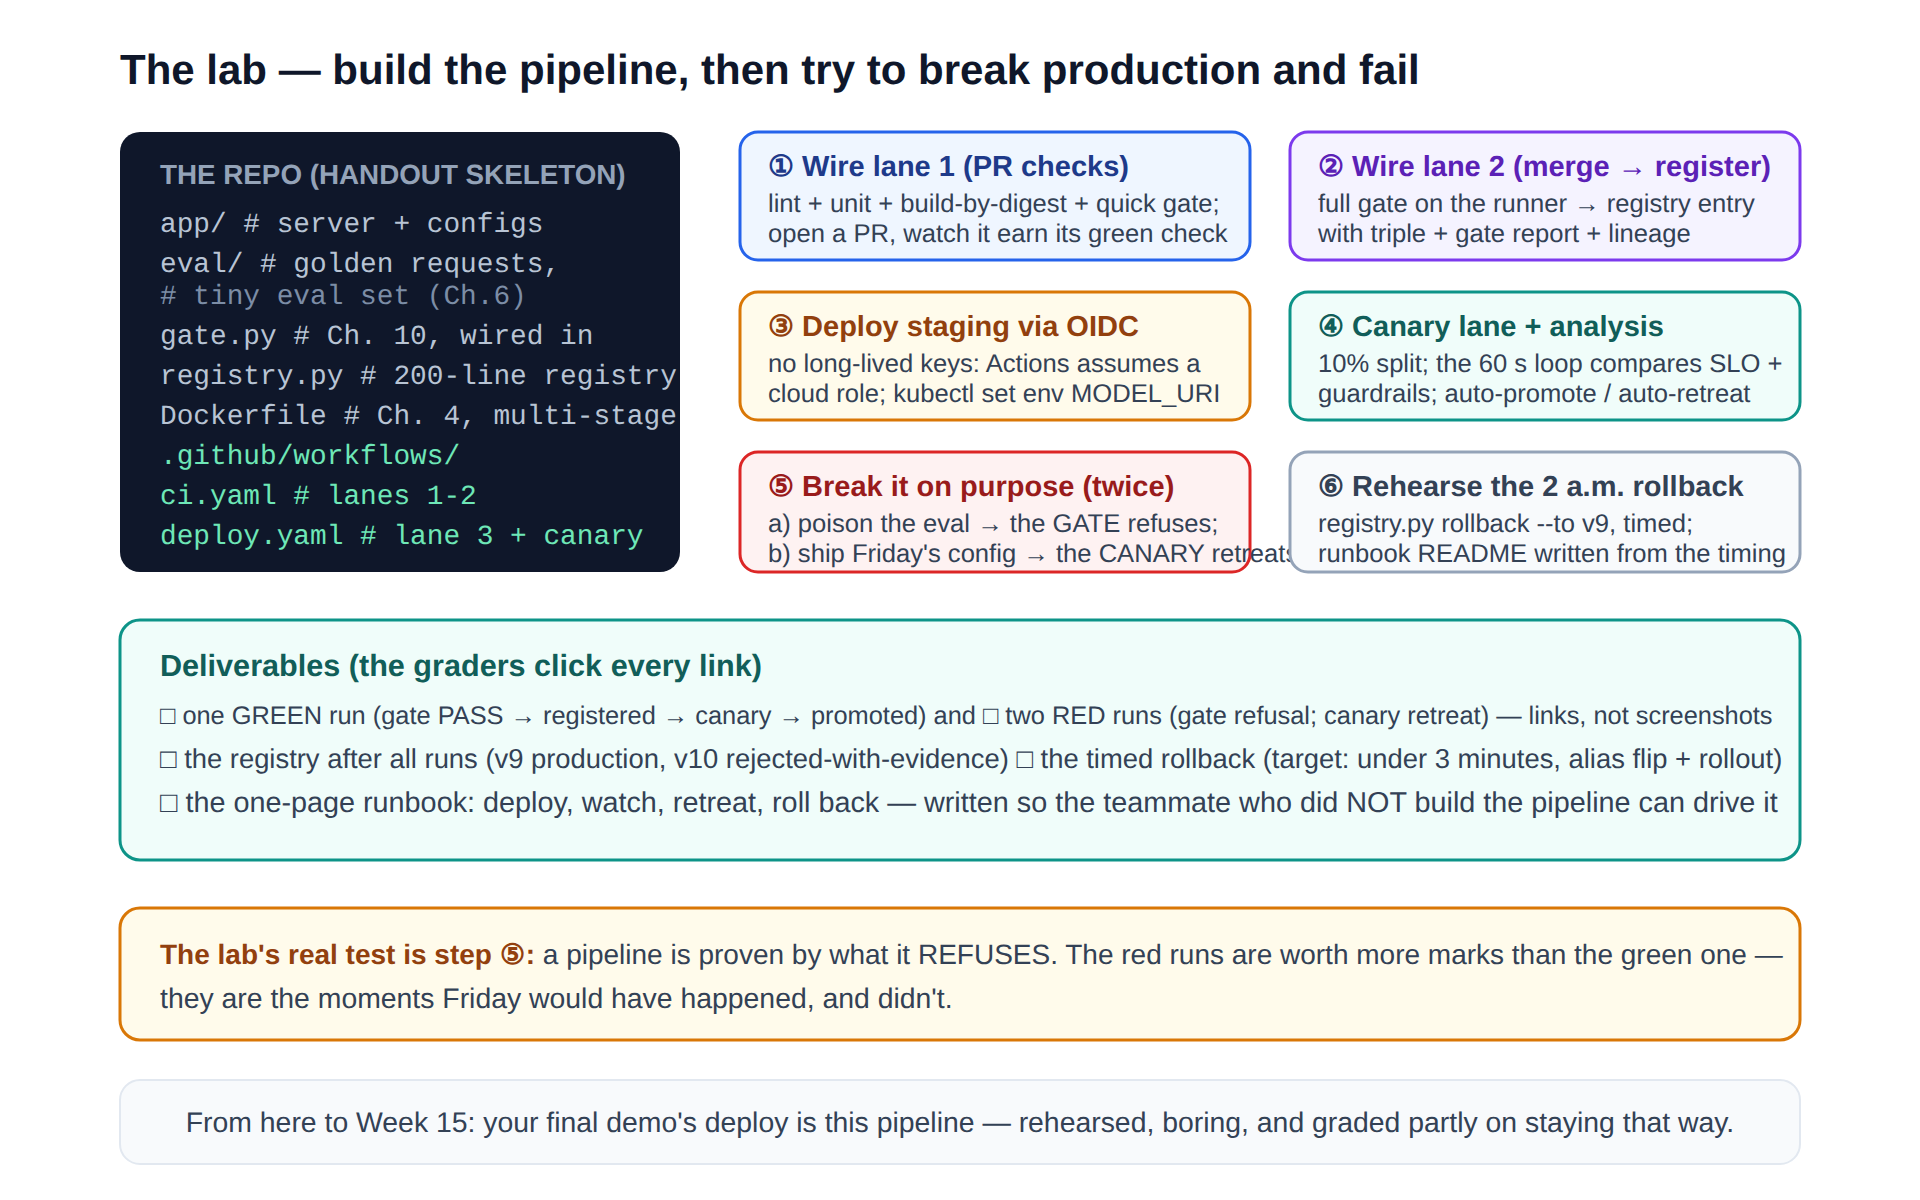
\includegraphics{figures/fig13-7_lab.png}}\\[3pt]
  \figcaption{그림 13-7  실습. 왼쪽은 교재에서 작성한 모든 것을 트리 하나에 모은 저장소 뼈대다. 오른쪽은 첫 PR부터 연습한 롤백까지 여섯 단계다. 아래의 제출물은 실행 링크이며 붉은 실행이 녹색 실행보다 중요하다.}
\end{tbbfigure}

\subsection*{여섯 단계}

\begin{tbbitemize}
  \item \textbf{① 경로 1을 연결한다.} 뼈대(app/, 골든 요청이 있는 eval/, gate.py, registry.py, Dockerfile, 워크플로 파일 두 개)를 포크한다. 간단한 PR을 열고 린트, 단위 테스트, \textbf{다이제스트로} 푸시하는 이미지 빌드, CPU에서 실행하는 빠른 게이트(골든 요청 + 200표본 평가)를 지켜본다. 기록 12-3처럼 로그를 읽는다. 이제 모든 단계가 이해되어야 한다.
  \item \textbf{② 러너를 등록하고 경로 2를 연결한다.} 실습 자료 스크립트가 T4를 \code{gpu} 태그 자체 호스팅 러너로 등록한다. systemd 서비스 하나이며 스팟에 적합하다. PR을 병합하고 내보내기 → 동등성 → 양자화+보정 → \textbf{게이트} → 스모크 스윕 → \code{registry.py register v10 --stage staging}을 지켜본다. 레지스트리 항목에 삼중항, 게이트 보고서, 계보 다이제스트가 있는지 확인한다.
  \item \textbf{③ OIDC로 스테이징에 배포한다.} 어디에도 장기 키를 두지 않는다. 워크플로는 OIDC(\code{permissions: id-token: write})로 클라우드 역할을 맡은 뒤 \code{kubectl set env … MODEL\_URI=\$(registry.py resolve chat/\allowbreak staging)}를 실행한다. 제6장의 환경 변수 배포(기록 6-7)를 이제 범위가 제한되고 몇 분만 유효한 자격 증명을 가진 로봇이 입력한다.
  \item \textbf{④ 경로 3인 카나리를 연결한다.} \code{deploy.yaml}이 \code{canaryTrafficPercent: 10} 또는 실습 자료의 원시 Deployment 가중 Service 변형을 패치한 뒤 40줄 분석 루프를 실행한다. 60초 창 다섯 개에서 SLO 조항 + 가드레일 네 개(답변 길이, 거부, 형식, 반복)를 동시 기준선과 비교한다. 판정에 따라 별칭을 전환해 승격하거나 카나리 0\%로 후퇴하고 그래프가 있는 PR 댓글을 남긴다. 무해한 v10으로 녹색 실행을 한 번 만든다.
  \item \textbf{⑤ 의도적으로 두 번 깨뜨린다.} (a) 골든 요청 하나의 기대 형식을 오염시키고 푸시한다. \textbf{경로 1에서 게이트가 거부}하며 회색 병합 버튼을 스크린샷으로 남긴 뒤 되돌린다. (b) 금요일을 재현한다. \code{max\_tokens: 256} 설정을 배포한다. 게이트는 긴 글을 생성하지 않아 통과한다. 승격하면 답변 길이 가드레일 때문에 \textbf{카나리가 약 3번째 창에서 후퇴}한다. PR 댓글을 저장한다. 자신이 만든 메커니즘으로 사례 13-A를 물리친 결과다.
  \item \textbf{⑥ 새벽 2시 롤백을 연습한다.} 좋은 v10을 승격한 상태에서 \code{registry.py rollback chat --to v9}를 실행하고 별칭 전환부터 v9이 처음 요청을 서빙할 때까지 \textbf{시간을 잰다.} 목표는 3분 아래다. 하한은 §12.3의 탄생이며 사전 워밍업이 이를 어떻게 바꾸는지 런북에서 논한다. 배포, 관찰, 후퇴, 롤백을 담은 한 쪽짜리 런북을 작성해 파이프라인을 \textit{만들지 않은} 팀원도 운전할 수 있게 한다. 그 팀원이 서명한다.
\end{tbbitemize}

\begin{calloutbox}{tbbred}{tbbxFEF2F2}
{\normalsize\bfseries\color{tbbx991B1B}상자 13-1  배포 위험 신호 — 공개 점검표}\par\vspace{3pt}
\begin{tbbitemize}
  \item \textbf{노트북에서 프로덕션으로 kubectl 실행} — 파이프라인만 작성자이고 사람은 PR과 승인을 작성한다.
  \item \textbf{배포 경로 어디서든 `:latest` 또는 다시 태그할 수 있는 참조 사용} — 다이제스트가 아니면 배포하지 않은 것이다. 제4장의 규칙은 계속 적용된다.
  \item \textbf{"비상용" 게이트 생략 플래그} — 비상 경로는 더 빠른 카나리이지 검사를 건너뛰는 것이 아니다.
  \item \textbf{자동 분석 없는 카나리} — 아무도 판정하지 않는 10\% 트래픽은 카나리가 아니라 사용자의 10\%가 베타 테스트하는 것이다.
  \item \textbf{연습하지 않은 롤백} — 금요일의 12분은 프로덕션에서 첫 연습을 한 대가였다.
  \item \textbf{릴리스 밖의 설정} — 변경해도 버전이 오르지 않는다면 반드시 자신의 사례 13-A가 된다.
  \item \textbf{저장소 시크릿의 장기 클라우드 키} — OIDC가 있다. 유출된 키는 회사 로고를 붙인 Knight의 여덟째 서버다.
\end{tbbitemize}
\end{calloutbox}

\vspace{3.0pt}

\begin{calloutbox}{tbbteal}{tbbxF0FDFA}
{\normalsize\bfseries\color{tbbx115E59}상자 13-2  런북 템플릿 — 이 페이지를 그대로 사용하라}\par\vspace{3pt}
\textbf{배포} — main에 병합하면 경로 2가 vN을 staging에 자동 등록한다. 승격하려면 승격 PR(\code{registry.py promote chat vN --request})을 열고 승인 하나를 받아 병합한다. 경로 3이 카나리를 실행하고 직접 별칭을 전환한다. \textit{kubectl은 입력하지 않는다.}

\textbf{관찰} — 카나리 중에는 Actions 실행의 실시간 로그나 \code{watch registry.py status chat}을 본다. 후자는 별칭, 카나리 비율, 현재 창 판정을 보여 준다. 승격 후에는 제14장 대시보드를 본다. 그전까지는 /metrics + \code{eval/\allowbreak watch.py}의 가드레일 스크립트를 사용한다.

\textbf{후퇴}(카나리가 이상하지만 아직 실패 판정 전) — \code{gh run cancel <id>}로 분석을 중단하고 카나리를 0으로 만든다. 별칭은 움직이지 않았으므로 언제든 안전하다.

\textbf{롤백}(나쁜 릴리스가 이미 승격됨) — \code{registry.py rollback chat --to <last-good>}를 실행한다. \code{registry.py list chat}의 이전 \code{production} 행에서 대상을 찾는다. 전환 ≈ 0.4 s, 플릿 수렴 ≈ 2–3 min이다. §12.3의 탄생이 하한이고 사전 워밍업이 줄인다. 이어 릴리스의 레지스트리 항목에 사고 메모를 기록하고 수정 PR을 연다. 프로덕션을 손으로 패치하지 않는다.

\textbf{담당자} — 승격 승인자는 [팀 목록] 중 아무 두 명이다. 02:00 규칙에 따라 온콜은 혼자 롤백할 수 있다. 이미 모든 검사를 통과한 릴리스를 다시 가리키므로 롤백은 구조적으로 사전 승인되었다. 승격은 낮까지 기다린다.

\textit{파이프라인을 만들지 않은 팀원의 서명: \_\_\_\_\_\_\_\_\_\_\_ (서명이 테스트다).}
\end{calloutbox}

\vspace{3.0pt}

제출물은 채점자가 클릭할 수 있는 \textbf{스크린샷이 아닌 링크}다. 승격 릴리스로 끝나는 경로 1→2→3의 녹색 실행 하나, 증거가 있는 붉은 실행 두 개(게이트 거부, 카나리 후퇴), 프로덕션의 v9과 증거와 함께 거부된 오염 후보를 보여 주는 레지스트리 목록, 시간을 잰 롤백 그림, 서명된 런북이다. 일찍 끝난 팀은 30분 미러링 트래픽을 위한 섀도 단계를 추가하고 출력을 비교한다. 이어 제14장 첫머리를 읽어 보자. 카나리의 분석 창이 곧 영구적이 되고 \textbf{모니터링}이라는 이름을 얻는다.

\begin{calloutbox}{tbbpurple}{tbbpurplefill}
{\normalsize\bfseries\color{tbbpurple}생각해 보기}\par\vspace{3pt}
\begin{tbbitemize}
  \item ⑤(b)의 카나리는 3번째 창(\textasciitilde{}3 minutes)에서 금요일 버그를 잡았다. 10\% 트래픽과 측정한 요청률에서 노출을 계산하라. 이어 신중한 팀을 위해 첫 창 1\%, 지수 단계 증가(1→5→25→100), 각 단계 10창 체류로 다시 설계하라. 전체 승격까지 시간 비용은 얼마이며 언제 이런 신중함이 가치 있는가?
  \item 런북의 롤백 하한은 §12.3의 탄생(\textasciitilde{}150 s)이다. 팀원이 승격 후 한 시간 동안 이전 릴리스를 블루/그린 방식으로 따뜻하게 유지하자고 제안한다. §12의 계산으로 가격을 매기고 얻는 롤백 시간을 제시하라. 한 시간이 올바른 창인가? 제14장의 어떤 데이터로 조정할 수 있는가?
  \item 실습 레지스트리는 저장소에 있는 JSON 200줄이다. 팀 규모에서 먼저 나타날 실패 유형 세 가지인 동시 쓰기, 인증, 감사 변조 등을 나열하고 무엇이 가장 먼저 실제 레지스트리 서비스로 이동하게 만드는지 설명하라.
  \item 프로젝트의 경로 3 승인 정책을 작성하라. 누가 승격을 승인할 수 있고 PR에 게이트 보고서, 카나리 계획, 롤백 담당자 중 어떤 증거를 인라인으로 보여 주어야 하는가? 02:00에 승인자가 잠들어 있으면 어떻게 하는가? §13.1 생각해 볼 문제의 2주 릴리스 위원회를 다시 만들지 않으면서 Knight의 교훈을 인코딩하라.
\end{tbbitemize}
\end{calloutbox}

\namedsection{요약}{열다섯 가지로 정리한 이 장}

\qitem{1}{\textbf{잘못된 배포는 부주의한 사람보다 빠진 제도에서 비롯된다.} 사례 13-A에는 완벽한 모델, 릴리스 밖의 설정, 초록색 대시보드, 전체 사용자에게 영향을 준 37분, 발굴 작업이 필요했던 롤백이 있었다. 엔지니어 한 사람을 고치면 재발하지만 버전 관리 + 파이프라인 + 점진적 노출을 고치면 피해 사용자-분은 0.5로 줄어든다(74배).}

\qitem{2}{\textbf{Knight Capital은 이 문제의 대표 사례다.} 서버 여덟 대를 손으로 배포하다 한 대를 빠뜨렸고, 재사용된 플래그가 죽은 코드를 깨웠다. 45분 만에 4억 6천만 달러를 잃었으며 사고 중에는 어디에서 무엇이 실행되는지 아무도 몰라 첫 조치가 오히려 사태를 악화했다. §13의 모든 제목은 SEC 명령서에서 빠져 있던 제도 하나씩을 가리킨다.}

\qitem{3}{\textbf{배포 빈도는 허세가 아니라 안전이다(Flickr 2009 → DORA).} 드문 배포는 크고, 큰 배포는 연습되지 않았으며, 연습되지 않은 배포는 Knight가 된다. 네 숫자는 리드 타임(→22분), 배포 빈도(→병합마다), 장애 반경(→자동 후퇴를 포함한 10\%), 평균 복구 시간(MTTR, →2분짜리 별칭 전환)이다. 지루한 배포란 자동화되고, 버전이 붙고, 점진적이며, 되돌릴 수 있는 배포다.}

\qitem{4}{\textbf{릴리스는 증거를 갖춘 세 요소의 묶음이다.} 가중치 다이제스트 + 설정 다이제스트 + 이미지 다이제스트를 함께 고정하고, 허용 오차·슬라이스·평가 세트 다이제스트를 담은 게이트 보고서를 붙이며, 계보를 기록한다. 설정이 릴리스 밖에서 따로 이동했던 금요일의 버그는 이제 표현 자체가 불가능하다.}

\qitem{5}{\textbf{레지스트리는 바이트에 관한 약속을 담은 데이터베이스다.} 무엇이 실행 중이고 무엇이 안전하며 무엇이 바뀌었고 누가 만들었는지를 아무 정보 없는 터미널에서도 몇 초 안에 답할 수 있어야 한다. 제6장이 바이트를 보관했다면 레지스트리는 의미를 보관한다. MLflow든 클라우드 내장 기능이든 200줄짜리 JSON이든, 가치는 제품명이 아니라 스키마에 있다.}

\qitem{6}{\textbf{승격과 롤백은 같은 동작, 즉 포인터 이동이다.} 배포는 버전이 아니라 별칭(…/prod)을 참조한다. 전환은 0.4초, 플릿 수렴은 제5장의 롤아웃을 따라 약 2분이며 하한은 §12.3의 탄생 시간이다. 제4장 생각 상자의 답처럼 다시 태그하지 말고 다이제스트를 쓴다. 태그는 움직이지만 다이제스트는 움직이지 않는다.}

\qitem{7}{\textbf{파이프라인은 이미 가진 검사를 빠짐없이 치르기 위한 의식이다.} §7.6의 동등성, §10.3의 게이트, §9.5의 스윕, 제6장의 골든 픽스처를 모든 후보에 똑같이 실행하며 금요일이라고 건너뛰는 길은 없다. 제5장의 표현을 빌리면 원하는 상태를 작성하는 주체가 하나 더 생긴 셈이다.}

\qitem{8}{\textbf{모델 CI는 앱 CI와 네 가지가 다르다.} 판정은 버전이 붙은 평가 픽스처에 대한 허용 오차이고, 아티팩트는 GB 단위이므로 한 번 빌드한 다이제스트를 승격하며, 일부 단계에는 실리콘이 필요해 자체 호스팅 스팟 T4 러너를 쓴다. 마지막 검사는 실제 트래픽을 필요로 하는데, 이는 테스트가 아니라 배포 전략이다.}

\qitem{9}{\textbf{빨간 실행 결과가 제품이다.} 병합 버튼을 비활성화하는 게이트는 동료의 의견이 아니라 마흔 번의 초록 선례를 쌓은 검사다. 품질 논쟁이 인프라 문제가 되는 순간이다. 건너뛰지 말고, 검사와 배포 사이에 다시 빌드하지 말며, 첫날부터 cosign/SLSA로 아티팩트에 서명한다.}

\qitem{10}{\textbf{배포 전략은 답하려는 질문으로 고른다.} 롤링은 "부팅되는가?", 블루/그린은 플릿 비용 2배를 감수하고 "1초 안에 되돌릴 수 있는가?", 카나리는 "현실에서 망가졌는가?", A/B는 "사용자에게 더 나은가?", 섀도는 "실제로 내보냈다면 어떻게 행동했을까?"에 답한다. 섀도는 사용자 위험이 없지만 계산 비용이 2배이고 모든 부작용을 막아야 한다.}

\qitem{11}{\textbf{카나리는 Haldane의 새에 그 새를 은퇴시킨 감지기를 더한 것이다.} 실제 트래픽의 10\%를 대화 전체가 같은 모델로 가도록 세션 해시하고, 동시에 실행되는 기준선과 비교하며, 판정과 수초 안의 후퇴를 자동화한다. 게이트가 확인할 수 없는 실제 입력, 실제 통합(금요일의 문제), 실제 인프라, 실제 SLO를 검사한다.}

\qitem{12}{\textbf{가드레일 메트릭은 우수성이 아니라 행동을 지킨다.} 답변 길이, 거부율, 형식 유효성, 반복, 언어 일치는 "모델이 이상해졌다"를 60초 루프에서 저렴하게 감지하는 프록시다. SLO 조항은 시스템을, 가드레일은 행동을 지키고, 품질은 A/B가 판단한다.}

\qitem{13}{\textbf{A/B는 안전을 이미 확보했다고 전제하는 제품 도구다.} 며칠에서 몇 주 동안 균형 잡힌 버킷과 미리 등록한 제품 메트릭, 통계를 사용하며 게이트와 카나리를 통과한 후보에만 실행한다. A/B를 카나리와 혼동하면 안전은 느려지고 실험은 타당성을 잃는다.}

\qitem{14}{\textbf{관리형 엔드포인트는 사다리의 마지막 칸이다.} 변형과 트래픽 분할, 레지스트리, 가드레일을 체크박스로 제공한다. 같은 개념에 더 높은 가격을 내고 스택 통제권은 줄어든다. 자기 사용률로 가격을 계산해야 하며(§12.5의 원장), 어느 단계에서도 게이트, 픽스처, 계보, SLO 문장, 단위 경제성은 공급자에게 넘길 수 없다.}

\qitem{15}{\textbf{실습의 채점 기준이 이 장의 주장이다.} 초록 실행 한 번, 빨간 실행 두 번(게이트 거부와 카나리 후퇴), 시간을 잰 롤백 연습, 작성자가 아닌 사람도 실행할 수 있는 런북을 요구한다. 파이프라인은 무엇을 허용하느냐보다 무엇을 거부하느냐로 입증된다. 빨간 실행은 일어나지 않은 금요일 사고다.}

\namedsection{연습문제}{}

\subsection*{A. 객관식}

\qitem{1}{사례 13-A의 버그(max\_tokens=256)가 오프라인 게이트를 통과한 이유는?}

\begin{tbboptions}
  \item ① 게이트의 허용 오차가 너무 느슨했다.        ② 게이트가 교사 강제 평가만 채점하고 실제 배포한 설정으로 생성하지 않아 릴리스가 아니라 모델만 검사했다.
  \item ③ 평가 세트가 너무 작았다.        ④ 게이트가 잘못된 GPU에서 실행되었다.
\end{tbboptions}

\qitem{2}{이 장에서 말하는 "릴리스"는 무엇인가?}

\begin{tbboptions}
  \item ① 모델 가중치        ② Docker 이미지
  \item ③ 게이트 보고서와 계보를 포함해 고정한 가중치 + 설정 + 이미지 다이제스트의 세 요소        ④ prod 별칭이 가리키는 무엇이든
\end{tbboptions}

\qitem{3}{레지스트리 별칭을 이용한 롤백이 빠르고 안전한 주된 이유는?}

\begin{tbboptions}
  \item ① 준비 상태 프로브를 건너뛴다.        ② 결정, 무엇이 안전한지에 대한 지식, 실행 수단이 연습된 포인터 이동 하나로 합쳐지고, 수렴은 평소 제5장 롤아웃과 같기 때문이다.
  \item ③ 이미지 가져오기를 피한다.        ④ 별칭이 로드 밸런서를 우회한다.
\end{tbboptions}

\qitem{4}{Knight Capital의 첫 조치, 즉 정상 서버 일곱 대에서 새 코드를 롤백한 일이 상황을 악화한 이유는?}

\begin{tbboptions}
  \item ① 롤백이 너무 느렸다.        ② 재사용된 FLAG와 업데이트되지 않은 여덟 번째 서버의 죽은 코드가 트리거였고, 어디에서 무엇이 실행되는지 보여 주는 권위 있는 기록이 없었다.
  \item ③ 시장이 불리하게 움직였다.        ④ 새 코드는 사실 문제가 없었다.
\end{tbboptions}

\qitem{5}{모델 CI가 아티팩트를 한 번만 빌드한 뒤 환경 사이에서 다이제스트를 승격하는 이유는?}

\begin{tbboptions}
  \item ① 다시 빌드하면 느리다.        ② 검사와 배포 사이의 재구축은 모든 검사를 무효화하므로 게이트를 통과한 바이트가 실제 배포되는 바이트와 같아야 한다.
  \item ③ 레지스트리가 빌드마다 요금을 받는다.        ④ 다이제스트의 압축률이 더 좋다.
\end{tbboptions}

\qitem{6}{카나리가 어제의 메트릭이 아니라 동시에 실행되는 기준선과 비교하는 이유는?}

\begin{tbboptions}
  \item ① 어제의 데이터는 삭제되었다.        ② 트래픽에는 하루 주기의 성격이 있어(제12장) 같은 시간의 대조군만 릴리스 변화와 시각 효과를 분리할 수 있다.
  \item ③ Prometheus 보존 기간이 짧다.        ④ 오토스케일링 때문에 기준선이 드리프트한다.
\end{tbboptions}

\qitem{7}{카나리와 A/B의 차이를 올바르게 설명한 것은?}

\begin{tbboptions}
  \item ① 둘은 같은 말이다.        ② 카나리는 안전을 묻는 도구(몇 분, "망가졌는가?", 자동 판정)이고 A/B는 제품을 묻는 도구(몇 주, "더 나은가?", 통계)이며, A/B는 게이트와 카나리를 이미 통과했다고 전제한다.
  \item ③ A/B는 인프라용이고 카나리는 모델용이다.        ④ 카나리가 A/B보다 더 많은 트래픽을 필요로 한다.
\end{tbboptions}

\qitem{8}{섀도 배포에서 피할 수 없는 비용 두 가지는?}

\begin{tbboptions}
  \item ① 느린 롤아웃과 큰 이미지        ② 사용자가 체감하는 위험과 호출기 부하
  \item ③ 미러링한 트래픽 조각에 드는 약 2배의 계산 비용과 쓰기·청구·이메일을 비롯한 모든 부작용 차단        ④ 추가 레지스트리와 더 긴 게이트
\end{tbboptions}

\subsection*{B. 단답형}

\qitem{1}{사례 13-A에서 빠진 세 가지 제도와 각각을 구축하는 절을 말하자.}

\qitem{2}{평가 세트 자체에 버전과 다이제스트를 고정해야 하는 이유는 무엇인가? 누군가 그 자리에 "어려운 예제 몇 개만" 더하면 무엇이 조용히 깨지는가?}

\qitem{3}{모델 파이프라인의 세 경로를 트리거, 러너, 최종 상태와 함께 나열하자.}

\qitem{4}{생성형 카나리의 가드레일 메트릭 네 가지를 들고, 가드레일이라는 부류의 한 문장짜리 근거("행동의 동일성")를 설명하자.}

\qitem{5}{채팅 워크로드의 카나리 분할에 세션 해시를 사용하는 이유는 무엇인가? 요청마다 나눌 때 생기는 UX 실패와 메트릭 실패를 각각 말하자.}

\qitem{6}{긴급 배포 원칙("게이트를 건너뛰지 않는다. 긴급 경로는 더 빠른 카나리다")을 말하고, Knight 사고가 이 원칙을 어떻게 뒷받침하는지 설명하자.}

\subsection*{C. 논술형}

\qitem{1}{사례 13-A의 비난 없는 사후 분석을 작성하자. 시간선, 영향(피해 사용자-분), 사람 이름이 아니라 빠진 제도로 표현한 근본 원인, 담당자와 날짜를 포함해 §§13.2–13.4에 연결한 개선 조치를 담는다. 대부분의 사후 분석이 빼먹는 문단도 추가하자. 하지 않을 개선은 무엇이며, 재발 가능성에 비해 비용이 큰 이유는 무엇인가?}

\qitem{2}{다음 주장에 찬성하거나 반박하자. "레지스트리가 하중을 받는 핵심 제도이고 파이프라인과 카나리는 그 주위의 자동화다." 금요일 사고(레지스트리만으로 막을 수 있었는가?), Knight(가장 먼저 없었던 것은 무엇인가?), 새벽 2시 테스트를 근거로 쓰고, 스타트업에서 가장 먼저 만들 제도 하나와 나머지를 미뤄 받아들일 실패를 밝힌다.}

\qitem{3}{배포 전략을 설계하자. 팀은 (a) 매주 기반 모델 업그레이드, (b) 매일 프롬프트/설정 수정, (c) 분기마다 엔진 메이저 버전을 배포한다. 각각에 대해 경로, 전략 단계, 대기 시간, 가드레일을 포함한 전체 경로, 장애 반경 산술, 하한을 포함한 롤백 계획을 제시한다. 세 경로가 달라지는 모든 지점을 정당화한다.}

\qitem{4}{배포 관점의 자체 구축 대 외부 도입 논술이다. 자기 프로젝트 팀의 규모, 모델, 중간 점검에서 확인한 트래픽을 기준으로 KServe를 대상으로 하는 경로 1–3 파이프라인과 레지스트리 + 가드레일을 갖춘 SageMaker 엔드포인트를 비교하자. §12.5 원장으로 마진을 계산하고, 그대로 이전되는 요소(세 요소 묶음, 게이트, 픽스처)를 나열한 뒤 도입·보류·혼합 가운데 하나를 권고한다. 결론을 뒤집을 메트릭 하나로 끝맺는다.}

\namedsection{정답과 해설}{}

\subsection*{A. 객관식}

\qitem{1}{\textbf{②} 게이트의 사각지대는 구조적이었다. 게이트는 가중치를 평가했지만 실패는 실제 배포된 가중치 + 설정으로 이루어진 릴리스에 있었다. "배포하는 것을 검사하라"는 원칙 때문에 경로 2가 조립된 릴리스에 게이트를 적용하고 §13.4가 다시 카나리로 검사한다. (§13.1, §13.3)}

\qitem{2}{\textbf{③} ④는 순환 정의다. 별칭은 릴리스를 가리킬 뿐 릴리스를 정의하지 않는다. 이동하는 단위는 세 요소 + 증거이며, 이를 고정했기 때문에 금요일과 같은 버그를 표현할 수 없게 된다. (§13.2)}

\qitem{3}{\textbf{②} 속도보다 중요한 것은 결정 + 지식 + 수단이 한곳에 모인 연습된 일체성이다. 플릿 쪽 하한은 §12.3의 탄생 시간이므로 런북에서 이 시간을 측정한다. (§13.2)}

\qitem{4}{\textbf{②} 교훈은 절차보다 지식에 관한 것이다. "어디에서 무엇이 실행되는가"에 대한 권위 있는 기록이 없으면 조치는 추측이 되고, 실제로 그 추측이 트리거를 다시 작동시켰다. 레지스트리가 바로 그 권위다. (§13.1–13.2)}

\qitem{5}{\textbf{②} 파이프라인을 통과하는 동안 신원을 유지하는 것이 신뢰 사슬의 전부다. 게이트 → 레지스트리 → 배포가 같은 다이제스트를 참조하지 않으면 초록 검사는 실제로 배포되지 않는 바이트를 인증한다. (§13.3)}

\qitem{6}{\textbf{②} 제12장의 일간 곡선은 교란 변수다. 14:00과 03:00의 비교는 후보가 아니라 시계를 측정한다. 동시 대조군은 가장 저렴하면서 타당한 실험 설계다. (§13.4)}

\qitem{7}{\textbf{②} 서로 다른 질문에는 서로 다른 도구를 쓴다. 게이트 → 카나리 → A/B 순서는 과학보다 안전이 먼저라는 뜻이다. (§13.4)}

\qitem{8}{\textbf{③} 미러링한 조각은 실제 추론 자원을 소비하고(제12장에서 가격을 계산했다), 살아 있는 부작용을 가진 섀도는 연습이 아니라 두 번째 프로덕션이다. (§13.4)}

\subsection*{B. 단답형}

\qitem{1}{버전이 붙은 릴리스(§13.2, 레지스트리와 세 요소), 배포할 것을 검사하는 파이프라인(§13.3, 세 경로), 자동 후퇴를 포함한 점진적 노출(§13.4, 카나리)이다. (§13.1)}

\qitem{2}{게이트 판정은 "이 세트에서 Δ와 허용 오차의 비교"이므로 세트는 측정의 절반이다. 제자리에서 바꾸면 과거 모든 PASS/FAIL의 의미가 말없이 달라져 서로 다른 시험의 점수가 되고, 회귀 비교와 계보 고정이 깨진다. 새 예제에는 새 평가 세트 버전을 부여하고 기준선을 명시적으로 다시 정한다. (§13.3)}

\qitem{3}{경로 1: 모든 PR / CPU 러너 / 위생 검사 + 빠른 게이트 → 초록 검사. 경로 2: main 병합 / 자체 호스팅 GPU 러너 / 내보내기→양자화→게이트→스모크 테스트 → 증거가 붙은 등록된 스테이징 릴리스. 경로 3: 사람의 승인 / OIDC로 클러스터 접근 / 카나리 분석 → 자동 승격(별칭 전환) 또는 자동 후퇴. (§13.3)}

\qitem{4}{답변 길이 분포, 거부/사과 비율, 형식 유효성(JSON 파싱), 반복 점수에 언어 일치를 더할 수 있다. 근거는 배포의 귀무가설이 행동의 \textbf{동일성}이라는 데 있다. 가드레일은 "이상해짐"을 저렴하게 감지하고 실제 품질 판정은 A/B까지 기다린다. (§13.4)}

\qitem{5}{UX 측면에서는 한 대화가 여러 모델 사이를 오가며 중간에 성격이 흔들린다. 메트릭 측면에서는 같은 세션의 턴이 양쪽 집단에 들어가 두 모집단을 오염시키고 비교의 독립성을 무너뜨린다. 대화 ID를 해시한다(제11장의 어피니티 장치). (§13.4)}

\qitem{6}{긴급 상황은 \textbf{속도}만 바꾼다. 카나리 창을 줄이고 롤백을 미리 준비하며 호출 범위를 넓힐 수 있지만 \textbf{검사}는 바꾸지 않는다. 압박받을 때 검증되지 않은 변경이 가장 위험하기 때문이다. Knight의 배포는 마감에 쫓겨 수동으로 진행했고 검증도 롤백 준비도 없었다. (§13.3, §13.1)}

\subsection*{C. 논술형 채점 기준}

\qitem{1}{다음을 확인한다. 프로브와 대시보드가 무해하게 초록색이었던 두 지점을 포함한 분 단위 시간선, 막연한 표현이 아니라 피해 사용자-분 37로 계산한 영향, 릴리스 밖 설정을 정확히 지목하면서 사람 대신 제도로 표현한 원인, 각 절에 연결하고 이 실패 부류를 잡는 카나리 가드레일을 명시한 개선 조치, 그리고 납득할 수 있는 "하지 않을 일"이다. 예를 들어 전체 블루/그린은 §12의 비용을 계산한 뒤 한계 비용이 거의 없는 카나리에 비해 과하다고 기각할 수 있다. 비난하지 않으면서도 개선 조치의 \textbf{책임자}를 분명히 한 답이 최고 점수를 받는다. (§§13.1–13.4)}

\qitem{2}{좋은 글은 각 도구가 서로 다른 실패 부류에 답함을 알아본다. 레지스트리는 Knight에게 없었던 "어디에 무엇이 있는가"를 제공하는 지식의 바닥이지만, 금요일에는 카나리가 필요했다. 레지스트리는 나쁜 릴리스도 완벽하게 기록할 뿐이다. 무엇을 먼저 만들지에 대해서는 레지스트리(가장 저렴하고 연습된 롤백을 가능하게 함)와 카나리(투입 노력당 피해 사용자-분을 가장 크게 줄임) 모두 타당하다. 다만 미뤄서 감수하는 실패를 솔직히 밝혀야 한다. 레지스트리 우선이면 금요일 사고를 한 번 더, 카나리 우선이면 느린 롤백을 감수한다. (장 전체)}

\qitem{3}{세 경로는 실제로 달라야 한다. (a) 모델 계열 경계에서 섀도 + 긴 카나리 + 품질 주장을 위한 전체 A/B, (b) 경로 1 + 롤링 또는 빠른 카나리(설정 변경이지만 사례 13-A 때문에 가드레일 카나리는 유지), (c) 엔진에는 즉시 되돌릴 수 있고 인프라 위험에 맞지만 §12 기준 창 비용이 2배인 블루/그린 + 수치 검사용 섀도(§7.6/§10.4의 순서 변경 주의)다. 전략 이름만 나열하기보다 구체적인 체류 시간, 장애 반경 수치, 롤백 하한(§12.3)을 제시한 답을 높이 평가한다. (§13.4)}

\qitem{4}{원장에는 마진 × 인스턴스 시간과 절약한 SRE 시간을 함께 적어야 한다. 이전 가능한 아티팩트, 즉 세 요소, 게이트, 픽스처, 레지스트리 스키마와 그대로인 파이프라인 경로 1–2를 밝힌다. 바뀌는 것은 경로 3의 동사가 공급자 API 호출이 된다는 점뿐이다. 판정은 팀의 형태에 연결한다. 결론을 뒤집는 좋은 메트릭에는 모델×팀 증가(→관리형을 더 일찍 선택), 규모가 커졌을 때의 사용률(→자체 호스팅), 규정 준수 요구가 있다. 산술이 일관되면 어느 결론도 만점을 받을 수 있지만 홍보 문구를 옮겨 적으면 점수를 받지 못한다. (§13.5, §12.5)}

\namedsection{더 읽을거리}{}

\textbf{[이번 주]} 표시는 실습에 직접 도움이 되는 자료이고, \textbf{[N주 차]} 표시는 뒤에서 다시 가치가 커지는 자료다.

\begin{tbbitemize}
  \item \textbf{[이번 주] GitHub Actions 문서 — 워크플로 문법, 자체 호스팅 러너, 클라우드 공급자용 OIDC} — 실습을 떠받치는 세 페이지다. OIDC 안내서를 적용하면 프로젝트에 남은 마지막 장기 키를 없앨 수 있다.
  \item \textbf{[이번 주] MLflow Model Registry 문서(별칭, 단계, 계보)} — 이제 읽을 때가 된 제6장의 더 읽을거리다. UI를 갖춘 터미널 기록 13-1의 레지스트리 스키마라고 생각하자. 제품이 아니라 스키마로 읽는다.
  \item \textbf{[이번 주] Argo Rollouts 문서(카나리, 분석 템플릿)} — 제5장에서 예고한 후속 내용이다. 단계별 트래픽 가중치, Prometheus 기반 분석, 자동 롤백으로 §13.4를 컨트롤러로 구현한다.
  \item \textbf{Knight Capital 관련 SEC Administrative Order(2013)와 "Knightmare" 사후 분석 자료} — §13.1의 1차 자료다. 명령서의 조사 결과를 그림 13-3과 나란히 읽고 빠진 경로를 세어 보자.
  \item \textbf{J. Allspaw \& P. Hammond, "10+ Deploys per Day: Dev and Ops Cooperation at Flickr"(Velocity 2009)} — DevOps의 씨앗이 된 발표다. 지금도 온라인에서 볼 수 있다. 2009년의 고통 가운데 이 과정의 각 장이 제도로 바꿔 놓은 것이 얼마나 많은지 살펴보자.
  \item \textbf{Google SRE Workbook의 "Canarying Releases"} — §13.4를 성숙한 수준으로 다룬다. 모집단 선택, 메트릭 선택, 작은 카나리의 통계, 가드레일과 SLO의 차이를 프로덕션 수준의 깊이로 설명한다.
  \item \textbf{DORA의 "Accelerate: State of DevOps" 보고서} — §13.1의 네 숫자를 뒷받침하는 측정 프로그램이다. 거울처럼 사용해 과정 프로젝트를 솔직하게 채점하고 가장 약한 지표를 찾자.
  \item \textbf{[이번 주, 가볍게] 대형 OSS 모델 저장소의 Actions 탭(vLLM이 좋은 예다)} — 초록 실행 하나와 빨간 실행 하나를 처음부터 끝까지 읽어 보자. 이제 그 언어를 이해할 수 있다. 무엇에 게이트를 적용하고 무엇은 아직 손으로 배포하는지 확인한다.
\end{tbbitemize}

\vspace{5.0pt}

\begin{calloutbox}{tbbblue}{tbbbluefill}
{\normalsize\bfseries\color{tbbblue}다음 장 — 제14장: 모니터링과 신뢰성}\par\vspace{3pt}
카나리의 분석 루프는 다섯 창을 실행한 뒤 멈췄다. 하지만 그 루프가 물었던 "TTFT는 정직한가? 행동이 드리프트했는가?"라는 질문은 승격과 함께 만료되지 않는다. 프로덕션은 아무도 듣지 않는 청중을 향해 영원히 답을 내놓는다. 제14장은 그 청중을 상시 체제로 만든다. \textbf{Prometheus와 Grafana}는 제11장의 /metrics 줄과 이 장의 가드레일을 강의계획서에서 약속한 서빙 대시보드로 바꾼다. \textbf{경보}는 SLO 문장을 규칙으로 만들어 막연한 느낌이 아니라 소진율에 따라 호출기가 울리게 한다. \textbf{드리프트 탐지}는 어느 배포 게이트도 얼려 둘 수 없는 것, 즉 사용자 집단 하나씩 평가 세트에서 멀어지는 입력 분포를 감시한다. §12.4에서 예고한 전쟁 이야기도 돌아온다. 시간 분할 GPU의 설명되지 않는 p99를 실제 대시보드에서 해결한다. 실습에서는 대시보드와 경보를 구축하며, 파이프라인을 물려받은 온콜 담당자에게 마침내 계기판이 생긴다.
\end{calloutbox}
